\documentclass[
   catalan,
%   handout,
   ]{beamer}
\usepackage{babel}
\usepackage[utf8]{inputenc}
\usepackage[style=authoryear,sortcites=true]{biblatex}
\newcommand{\bibendash}{--}
\usepackage{cclicenses}
\usepackage{appendixnumberbeamer}
\usepackage{tikz}
\usetikzlibrary{shapes,arrows,positioning}
\usepackage{pgfplots}
%\usetikzlibrary{dateplot}  
%\usetikzlibrary{pgfplots.groupplots}






% \pgfplotsset{
%    rrbtimeseries/.style={
%         % date coordinates in=x,
%         ylabel=Temperature (K),
%         % legend style={font=\footnotesize},
%         % tick label style={font=\footnotesize},
%         % every axis x label/.style={
%         %   at={(1.3,0)},
%         %   anchor=north,
%         %   },
%         % label style={font=\footnotesize},
%         % xticklabel style= {rotate=17,anchor=north east},
% %        every axis title shift=0pt,
% %        max space between ticks=15,
%        %  every mark/.append style={mark size=6},
%        %  major tick length=0.1cm,
%        %  minor tick length=0.066cm,
%        %  very thin,
%        %  every axis legend/.append style={
%        %    at={(1.2,0)},
%        %    anchor=south east,
%        %    draw = none},
%        % legend columns = 4,
%        % unbounded coords=jump, %v>1.4
%     },

%   % rrbrs/.style={
%   %       rrbtimeseries,
%   %       width = \textwidth,
%   %       height = 0.25\textwidth,
%   %       every axis x label/.style={
%   %         at={(1.3,-1)},
%   %         anchor=north,
%   %         },
%   %       ylabel = {},  
%   %       max space between ticks=50,
%   %       every axis legend/.append style={
%   %         at={(1,-1.1)},
%   %         anchor=north east,
%   %         draw = none},
%   %       title style={font=\small,below,anchor=north,fill=white},
%   %   },
%  }




\pgfplotsset{
   timeseries/.style={
        date coordinates in=x,
        ylabel=Temperature (K),
        legend style={font=\footnotesize},
        tick label style={font=\footnotesize},
        every axis x label/.style={
          at={(1.3,0)},
          anchor=north,
          },
        label style={font=\footnotesize},
        xticklabel style= {rotate=17,anchor=north east},
%        every axis title shift=0pt,
%        max space between ticks=15,
        every mark/.append style={mark size=6},
        major tick length=0.1cm,
        minor tick length=0.066cm,
        very thin,
        every axis legend/.append style={
          at={(1.2,0)},
          anchor=south east,
          draw = none},
       legend columns = 4,
    },
    rd/.style={
        timeseries,
        every axis x label/.style={
          at={(1.3,-1)},
          anchor=north,
          },
        label style={font=\footnotesize},
        ylabel = {},
        width=17cm,
        height=3.5cm,   
        max space between ticks=50,
        every axis legend/.append style={
          at={(1,-1.1)},
          anchor=north east,
          draw = none},
        title style={font=\small,below, at={(0.7,1.7)},anchor=north,fill=white},
    }
}


%        unbounded coords=jump, %v>1.4
%        unbounded coords=discard, %v>1.4


%http://tex.stackexchange.com/questions/46422/axis-break-in-pgfplots

%http://tex.stackexchange.com/questions/52409/insert-a-separate-mark-inside-a-pgfplots-graph


\mode<beamer>
{
  \usetheme{Madrid}
  \setbeamercovered{transparent}
  \beamertemplatenavigationsymbolsempty
}

\mode<handout>
{
  \usepackage{pgfpages}
  \pgfpagesuselayout{8 on 1}[a4paper,border shrink=5mm]
  \setbeamercolor{background canvas}{bg=black!5}
  \usetheme{Boadilla}
  \useinnertheme{default}
  \usecolortheme{dove}
}

\bibliography{../bibliografia}
\renewcommand*{\bibfont}{\footnotesize}
\bibparsep 0.2cm
\bibhang 0.25cm
%\ExecuteBibliographyOptions{
%  isbn=false,url=false,doi=false,firstinits=true,abbreviate=true
%}


%------------- capçaleres pdf -----------

\title%
   [Model multiresolució per a sèries temporals]%
   {Disseny i modelització d'un sistema de gestió multiresolució per a sèries temporals}

\author[A. Llusà]
{%
  Aleix Llusà Serra \\
  {\footnotesize Direcció: Teresa Escobet Canal i Sebastià Vila-Marta}
}

\institute[Programa doct.\ ARV UPC]
{
  {\large Universitat Politècnica de Catalunya} \\
  Programa de Doctorat en Automàtica, Robòtica i Visió 
}


\date[Setembre 2015]
{Tesi Doctoral \\ Setembre 2015}


\subject{Defensa de tesi doctoral 2015}
\keywords{sèries temporals; model de dades; sistemes de bases de dades; sistemes de monitoratge}



\begin{document}

\begin{frame}[plain]
 \titlepage

 \begin{center}
   {\footnotesize \cc\bysa}
   {\tiny Aquest document està sotmès a una llicència de Reconeixement-CompartirIgual 3.0 de Creative Commons\\
     El codi font \LaTeX\ del document es troba a
     \url{http://escriny.epsem.upc.edu/projects/rrb/} }
  \end{center}

\end{frame}

\section*{Índex}
\begin{frame}{Índex}
 \tableofcontents
\end{frame}


% \section{Introducció}
% \begin{frame}{Introducció}

\begin{itemize}

  \item Anàlisis de sèries temporals. Multitud de metodologies i algoritmes.

  \item Sistemes de gestió de bases de dades (SGBD). Estructuració de
    les dades i integració de les operacions.

  \item Necessitat de coneixement entre SGBD i sèries
    temporals \parencite{stonebraker09:scidb,zhang11}

  \item Els SGBD aplicats a les sèries temporals tenen aspectes propis
    que els converteixen en objecte d’estudi

  \item Proposem dissenyar un model de SGBD multiresolució per tal
    d'emmagatzemar les sèries temporals de forma compacta i poder-les
    consultar amb la resolució desitjada, ja que és una aplicació
    habitual

\end{itemize}






\end{frame}






%%% Local Variables: 
%%% mode: latex
%%% TeX-master: "presentacio"
%%% End: 


% \section{Estat de l'art}
% \todo{dir}
dir que en el nostre model no ens ocupem de l'etapa d'adquisició/mostreig de les sèries temporals sinó que tenim unes mesures que s'han capturat d'alguna manera. Si bé cal destacar que alguns SGST sí que influeixen al procés d'adquisició, per exemple poden controlar obtenir més mostres si veuen coses rares, no mostrejar més si és tranquil, canviar paràmetres, etc.


\todo{}
explicar el data mining com a background per a les oepracions que es poden fer amb les sèries temporals: pattern search, similiraties, etc.

\section{Sèries temporals}





Una sèrie temporal és un conjunt de valors cadascun dels quals té
associat un instant de temps diferent.  Tradicionalment s'anomenen
sèries temporals tot i que també s'accepta la denominació de
seqüències temporals, per exemple a \cite{last:hetland}.

Les sèries temporals s'emmarquen dins l'àmbit més genèric del que es
coneix com a \emph{dades temporals}. Les dades temporals són
co\l.leccions de dades arbitràries que estan associades a la dimensió
temps.  Dins del concepte de dades temporals s'hi encabeixen
co\l.leccions de dades de diversa natura. En funció de com un valor
queda vinculat amb el temps, es poden diferenciar dues
categories \parencite{assfalg08:thesis}.
\begin{enumerate}
\item La primera la formen les sèries temporals tal i com s'han
  definit prèviament, en la qual la dada està associada a un instant
  de temps.
\item La segona, que anomena \emph{bitemporal data}, la formen
  co\l.leccions de dades en que cada element té dos atributs
  temporals: el rang de validesa, que indica l'intèrval de temps en
  que la dada és vàlida, i el temps de transacció, que indica quan es
  va desar la dada a la base de dades.  
  %\citeauthor{assfalg08:thesis} a \cite{assfalg08:thesis} assegura que aquesta categoria de dades temporals es poden expressar en termes de la primera.\todo{Teresa5}
\end{enumerate}
Aquestes dues categories de dades temporals, tot i tenir aspectes en
comú, no poden ser tractades amb els mateixos
sistemes, \parencite{schmidt95}.


Les sèries temporals s'utilitzen en camps molt diversos i amb
objectius molt diferents. L'ús generalitzat és per a l'anàlisi i la
comprensió del comportament temporal de variables. L'evolució d'una
sèrie temporal es pot representar amb un model. Aquests models, en
l'àmbit de l'enginyeria, permeten realitzar tasques relacionades amb
validació de dades, diagnòstic i prognosis.  Per exemple, trobem
aplicacions de sèries temporals en el camp de l'avaluació de la
degradació de components \parencite{yu11}, anàlisi de l'estat dels
sensors d'un vaixell \parencite{palmer07}, validació i reconstrucció
de dades en xarxes de distribució d'aigua \parencite{quevedo10},
classificació de valors econòmics \parencite{dreyer95}, optimització
de la planificació semafòrica \parencite{last11}, estimació del temps
de viatge en autopistes \parencite{soriguera10} o transmissió
d'informació en xarxes de
sensors \parencite{jainagrawal05,yaogehrke02}.
\todo{també sèries temporals van de bracet amb GIS, exemple en dades hidrològiques [bollaert06:thesis]}


Aquest apartat té com a objectiu mostrar l'estat de l'art dels
principals processos vinculats en el treball amb sèries temporals. A
tal efecte s'organitza en tres subapartats.
 

El primer subapartat se centra en l'adquisició de dades. El primer
requeriment d'una sèrie temporal és l'adquisició de dades. Els
sistemes de monitoratge s'encarreguen de recollir dades dels sensors,
periòdicament o en base a esdeveniments.  Els problemes que es donen
durant l'adquisició generen defectes específics en les sèries
temporals que cal analitzar i tractar convenientment.


El segon subapartat tracta de l'anàlisi de sèries temporals, que és
la formalització de les tècniques que s'utilitzen per extreure
informació. A vegades aquesta extracció també es coneix com
descobriment de coneixement i s'emmarca dins de l'inte\l.ligència
artificial.


El tercer subapartat es dedica als sistemes d'emmagatzemat de sèries
temporals. L'emmagatzematge de les dades i la implementació de les
tècniques d'anàlisi té lloc en els sistemes de gestió de bases de
dades. Aquests s'encarreguen de l'organització correcte de la
informació i de respondre a les operacions de consulta. Les sèries
temporals necessiten un tractament específic per part d'aquests
sistemes.






\subsection{Adquisició de sèries temporals}

Els sistemes de monitoratge són un part important d'interacció entre
un procés i els usuaris, entenent com a procés qualsevol sistema
físic, químic, ambiental, etc.\ del qual es pugui recollir informació
continuada, ja sigui de forma periòdica o en funció
d'esdeveniments. Principalment, aquests sistemes s'encarreguen de
recollir dades, conèixer l'estat actual del procés i informar a
l'usuari. Els sistemes de monitoratge constitueixen la part principal
dels sistemes SCADA (\emph{Supervisory Control And Data
  Acquisition}). Un SCADA és el sistema encarregat de recollir i
centralitzar les dades de manera periòdica en el temps.



\begin{figure}[tp]
  \begin{center}
    \scriptsize 
    ../../../imatges/aplicacions/monitoratge.tex
  \end{center}
  \caption{Sistema de monitoratge: de l'adquisició de dades fins a informar l'usuari}
  \label{fig:sistema_monitoratge}
\end{figure}


El monitoratge es pot dividir en diferents blocs principals, els quals
es mostren a la \autoref{fig:sistema_monitoratge}. Un monitor
adquireix dades dels sensors. Les dades poden ser valors de mesures o
estats del procés adquirits com a esdeveniments. Fent referència a la
classificació de dades temporals de \textcite{assfalg08:thesis}, en
general les mesures es poden entendre com a sèries temporals i els
esdeveniments com a dades bitemporals.

En el cas de sistemes controlats o automatitzats, les dades adquirides
poden ser utilitzades per comandar o modificar el funcionament del
procés. Aleshores s'incideix en diferents nivells des de llaços de
control modificant directament un accionament, fet que no sol ser
habitual ja que els llaços de control solen realitzar-se els sistemes
electrònics que resideixen prop dels sistemes controlats, fins a
gestió de modes de funcionament i coordinació entre màquines, fet més
habitual.

L'ús generalitzat dels sistemes de monitoratge és el de proporcionar
informació de l'estat actual del procés. També disposen de la
possibilitat de generar alarmes senzilles com per exemple que no s'han
pogut adquirir les dades o que el sensor ha assolit un valor
crític. Per a usuari ens referim tant a un usuari humà com a un altre
sistema supervisor dotat amb inte\l.ligència artificial.

Per a càlculs més complicats amb les dades, els sistemes de
monitoratge utilitzen sistemes de gestió de bases de dades
(SGBD). Mitjançant els SGBD, s'emmagatzemen les dades en bases de
dades i posteriorment l'usuari les consulta per observar els històrics
o per obtenir informació i elaborar coneixement a partir de les dades
emmagatzemades.

La \autoref{fig:sistema_monitoratge} presenta una visió centralitzada
de l'adquisició de dades. Ara bé, els sistemes de monitoratge
internament poden tenir estructura distribuïda quan els sensors tenen
suficient capacitat de processament, com per exemple les xarxes de
sensors. En aquests casos els monitors cedeixen parts al sensors,
sobretot pel que fa als SGBD que passen a tenir un paper més rellevant
en la comunicació.


Un dels camps recents on l'adquisició de sèries temporals hi juga un
paper fonamental és el de les xarxes de sensors. L'abaratiment del
maquinari permet monitorar el procés amb grans quantitats de sensors
inte\l.ligents \parencite{jainagrawal05,yaogehrke02}, els quals tenen
processador i ràdio incorporats però tenen recursos limitats pel que
fa a transmissió, energia i processament i estan sotmesos a la
incertesa dels sensors. Així doncs, el problema de les xarxes de
sensors rau en estudiar l'ús eficient d'aquests recursos, pel qual
actualment trobem dues propostes.  Una solució consisteix en
transmetre la informació a un node central comprimint-la tant amb
agregacions (estadístics) com amb
aproximacions \parencite{deligiannakis07}.  Una altra solució
consisteix en tenir les dades distribuïdes en diferents sensors i
decidir com s'ha de resoldre cada consulta tenint en compte que el
processament local és més barat que la
comunicació \parencite{yaogehrke02,gehrkemadden04,bonnet01}.

\todo{el tema d'agregar informació en xarxes de sensors és interessant, potser hauria de tenir una secció pròpia}

\todo{citar kim12}:
Research Article
Aggregate Queries in Wireless Sensor Networks
Jeong-Joon Kim,1 In-Su Shin,1 Yan-Sheng Zhang,2 Dong-Oh Kim,3 and Ki-Joon Han1
Hindawi Publishing Corporation
International Journal of Distributed Sensor Networks
Volume 2012, Article ID 625798, 15 pages
doi:10.1155/2012/625798





\subsubsection{Problemes en el monitoratge}

Els sistemes de monitoratge habitualment presenten problemes derivats
de la reco\l.lecció de dades. Principalment distingim tres problemes.

\todo{parlar també del problema de la sincronització de rellotges}
\textcite[cap.~3]{kopetz11:realtime}


\begin{enumerate}
\item El primer problema és la gestió d'una quantitat enorme de dades. 

Un sistema de monitoratge recull una gran quantitat de dades. Ara bé, l'usuari només en pot observar una petita part sincronitzat (\emph{online}) amb el procés i les dades emmagatzemades esdevenen massa grans per a ser processades posteriorment \parencite{keogh97}. No obstant, les dades han de ser analitzades ja que contenen informació interessant per a les aplicacions de les sèries temporals descrites a l'apartat anterior. S'observa que en el context de monitoratge les dades recollides es poden considerar com a sèries temporals ja que abstractament són una co\l.lecció de mesures.


\item El segon problema és el de la necessitat de censurar les dades, és a dir validar que les dades siguin correctes i en cas contrari rebutjar-les o reconstruir-les. 

\textcite{quevedo10} mostren la quantitat d'informació que hi ha en els sistemes complexos de telecontrol. Aquesta informació s'obté de diversos sensors distribuïts pel camp de mesura.
En el moment de reco\l.lecció de dades apareixen dos problemes: valors que en un instant de temps prefixat no s'han pogut recollir i valors que són falsos. En el procés de gestió de dades no es poden emmagatzemar les dades amb aquests dos tipus de problema ja que aleshores els registres històrics serien inconsistents. 
Així doncs, cal comprovar que les dades emmagatzemades són correctes, mitjançant un procés de validació, i modificar-les en el cas que siguin falses, mitjançant un procés de reconstrucció que estimi els valors correctes. Per exemple, \citeauthor{quevedo10} apliquen aquests processos de validació i reconstrucció a xarxes de distribució d'aigua.


\item El tercer problema es dóna quan el període de mostreig no és regular, és a dir que les dades no es recullen de manera uniforme en el temps, però les aplicacions no ho contemplen o volen treballar amb dades a intervals regulars, també anomenat dades equi-espaiades.

Una causa de la irregularitat es deu a que els sistemes de monitoratge informàtics sovint no són capaços de complir amb exactitud el temps de mesura sinó que presenten una certa variació, ja sigui deguda a retards en els sensors, les comunicacions o la planificació del monitoratge amb altres tasques concurrents del sistema operatiu. Aquesta causa, però, es pot atenuar si els sensors envien el temps de mesura juntament amb el valor mesurat. Aleshores, el problema recau en la sincronització dels rellotges dels sensors. \todo{busca jitter en el periodic sampling de control}

Una altra causa es deu a que l'adquisició de dades prové de processos sotmesos a sistemes de control, els quals prenen el control de l'adquisició de dades. És a dir, el sistema de monitoratge ha d'obeir a les restriccions de temps imposades pels llaços de control. Aquestes restriccions són especialment crítiques en els sistemes de control en temps real ja que, aleshores, el sistema de monitoratge no pot imposar restriccions de temps diferents de les que s'han calculat per als llaços de control.  \textcite{lozoya08} mostren que s'ha de vigilar amb les entrades i sortides de les tasques periòdiques als sistemes en temps real. L'actuació dels sistemes de control es degrada quan no es té en compte que les operacions d'entrada i sortida estan subjectes a fluctuacions degudes al mostreig i a latències. Aquest problema afecta als sistemes de monitoratge en dues vessants.
Per una banda, els sistemes de monitoratge tenen una part de l'adquisició controlada per les aplicacions de control en temps real i per tant el període de mostreig resultant que veu el monitor no és regular. 
Per altra banda, les aplicacions que analitzen les dades obtingudes del monitoratge poden veure com la seva actuació es degrada si no consideren que l'adquisició de dades és irregular, el qual és similar a la regressió que s'observa \parencite{lozoya08} quan en el disseny d'un controlador discret es considera que es mostreja i s'actua periòdicament però en la implementació amb un sistema en temps real aquest pot fluctuar la periodicitat.
\todo{event based sampling/control}

\end{enumerate}



En conclusió, per tal de gestionar la complexitat derivada de la recollida de dades i també la complexitat de les consultes posteriors per part de l'usuari, els sistemes de monitoratge es recolzen en sistemes de gestió de bases de dades per gestionar l'emmagatzematge de les dades i la recuperació d'informació.





\subsection{Anàlisi de sèries temporals}

\todo{dir que una aplicació emergent és l'anàlisi de dades en temps real/en línia amb el procés per a prendre decisions}

L'anàlisi de sèries temporals consisteix en l'aplicació de
metodologies i d'algoritmes que permeten tasques com per exemple
l'extracció de característiques o obtenció de models.  Aquestes
tècniques es recullen en el que es coneix amb el nom de mineria de
sèries temporals (\emph{time series data mining}). La mineria de
dades, en la qual s'inscriu la de sèries temporals, és l'estudi
d'algoritmes específics per a extreure patrons de comportament de les
dades i s'inclou com un pas del procés general de descobriment de
coneixement a les bases de dades (\emph{knowledge discovery in
  databases}) \parencite{fayyad96,last01}.
% [M. E. Mueller, Relational Knowledge Discovery, Cambridge 2012. sec1.1p7]
%knowledge discovery: process of extracting new knowledge from a set of data about that set of data, This means that the acquisition of new lnowledge requires us to build a new model of the data.
% Data mining: refers mostly to the extraction of parts of information with respect to a given model. 
%Exemple: correlació, si dues coses tenen correlació no vol dir que necessàriament hi hagi una dependència causal entre les dades.

Actualment, les sèries temporals es consideren com un dels deu problemes
prioritaris en la mineria de dades \parencite{yangwu06}. Tal com
esmenta \textcite{fu11} en un article recent, la recerca en mineria de
sèries temporals s'ha incrementat en la darrera dècada. L'objectiu
principal és reduir la mida de les sèries temporals per tal de
disminuir el temps de processat de les dades.  \citeauthor{fu11}
resumeix l'estat actual de la mineria de sèries temporals de forma
exhaustiva i conclou que encara queden molts problemes per investigar
i resoldre. La recerca en tasques de mineria ha estat intensa però es
necessita millorar la representació de sèries temporals, ja que es
considera el pas que redueix la mida de les dades.

Segons \textcite{keogh02}, les quatre tasques que centren l'atenció de
la recerca actual de sèries temporals són l'indexat (\emph{indexing}),
que treballa amb una estructura comprimida de les dades; l'agrupament
(\emph{clustering}), que agrupa les dades segons la similitud entre
elles per tal de descobrir patrons; la classificació
(\emph{classification}), que etiqueta les dades segons les
característiques que presentin; i la segmentació
(\emph{segmentation}), que parteix una sèrie temporal en
subseqüències.  A més, \citeauthor{keogh02} comparen alguns algoritmes
experimentals duts a terme en aquests camps per diversos
autors. Recomanen a la comunitat de mineria de sèries temporals que
segueixi el seu estudi com a punt de referència per avaluar el
rendiment d'algoritmes similars.

Un pas comú previ a les quatre tasques anteriors és el de representació de la sèrie temporal. Les sèries temporals són discretes, són valors en punts de temps discrets, i la representació és el model de funció que aproxima la sèrie temporal a la seva naturalesa contínua original. La mineria de sèries temporals aprofita la representació per reduir la mida de les sèries temporals.
La representació de sèries temporals a trossos lineals (PLR, \emph{Piecewise Linear Representation}) \parencite{keogh97,keogh98} {é}s la més habitual actualment per ser més propera als usuaris ja que la visió de l'ésser humà segmenta les corbes en línies rectes.
Després de definir la PLR, \textcite{keogh00,keogh01} exploren altres representacions de sèries temporals per tal de reduir la mida d'una sèrie temporal i poder-la indexar més fàcilment. Proposen dues tècniques eficients en el càlcul: la \emph{Piecewise Aggregate Aproximation} i la \emph{Adaptive Piecewise Constant Approximation}, ambdues basades en la representació a trossos constants de la sèrie temporal. 
D'aquestes dues tècniques, \citeauthor{keogh00,keogh01} conclouen que mantenen una bona aproximació a la sèrie temporal i que a més  tenen molt menys cost de càlcul que altres de més complicades, com ara la \emph{Discrete Fourier Transform},  la  \emph{Singular Value Decomposition} o la \emph{Discrete Wavelet Transform}.

\todo{arreglar perquè quedi ben explicat; després en el model fem menció d'aquestes representacions}

\todo{potser posar-ho a estat de l'art tot això?}


In the design of the attribute interpolation function we can interpret
a time series in different ways, that is what we call the
representation of a time series. Keogh et al.\ \cite{last:keogh} cite
some possible representations for time series such as \emph{Fourier
  Transforms}, \emph{Wavelets}, \emph{Symbolic Mappings} or
\emph{Piecewise Linear Representation} (PLR). This last is remarked as
the most used owing to the most common representation is with linear
functions \cite{keogh01}.


\todo{last01} també fa una mena d'agregacions amb l'objectiu de trobar un a funció que s'aproximi a un interval de la sèrie temporal. Seria un mètode d'agregació amb aproximació?


\paragraph{Representació de sèries temporals}

\textcite{last:keogh}, cita vàries representacions per les sèries temporals com per exemple \emph{Fourier Transforms}, \emph{Wavelets}, \emph{Symbolic Mappings} o \emph{Piecewise Linear Representation} (PLR), però assenyala aquesta última com la representació més utilitzada. 
La PLR, funció definida a trossos lineal, és l'aproximació d'una sèrie temporal $S$, de llargada $n$, amb $K$ segments rectes. Els segments podrien ser polinomis de qualsevol grau, però la manera més comuna de representar sèries temporals és amb funcions lineals, segons Keogh, \cite{keogh02}.
Per aproximar el segment $S(t_a,t_b]$ d'una sèrie $S$, Keogh defineix dues tècniques: interpolació lineal, la recta que connecta $t_a$ i $t_b$, i regressió lineal, la millor recta que aproxima per mínims quadrats el segment entre $t_a$ i $t_b$.

Però també es pot representar una sèrie temporal amb una funció graó (\emph{step} o \emph{staircase function}); és a dir, amb una funció definida a trossos constant (\emph{piecewise constant representation}).
La representació a trossos constant és utilitzada en electrònica als convertidors digital-analògic (DAC, \emph{digital-to-analog converter}). En aquest cas, un senyal discret es considera una sèrie temporal i per reconstruir el senyal continu típicament s'aplica el model de \emph{zero-order hold}, equivalent a la representació a trossos constant,  o el de \emph{first-order hold},  equivalent a la representació a trossos lineal.
El model de \emph{zero-order hold} consisteix en mantenir constant cada valor fins al proper. S'obté una representació a trossos constant que en electrònica s'anomena seqüència de pulsos rectangulars (\emph{rectangular pulses}).

%http://en.wikipedia.org/wiki/Piecewise

%http://ca.wikipedia.org/wiki/Funció_definida_a_trossos

%http://en.wikipedia.org/wiki/Rectangular_function

%http://en.wikipedia.org/wiki/Step_function

% Piecewise Aggregate Approximation (PAA) \cite{keogh00}: aproxima una sèrie temporal partint-la en segments de la mateixa mida i emmagatzemant la mitjana dels punts que cauen dins del segment. Redueix de dimensió $n$ a dimensió $N$

% Adaptive Piecewise Constant Approximation (APCA) \cite{keogh01}: com el PAA però amb segments de mida variable.




\subsection{Emmagatzematge i gestió de sèries temporals}


Els sistemes de gestió de bases de dades (SGBD) són els sistemes informàtics que s'encarreguen d'emmagatzemar informació i de permetre a l'usuari consultar-la. A la secció \ref{sec:art:sgbd} es descriu com es formalitzen els SGBD, en aquest apartat ens centrarem en les necessitats que tenen les sèries temporals dels SGBD.


Les sèries temporals es diferencien d'altres tipus de dades en que els seus valors són dependents d'una variable: el temps. Com a conseqüència, qualsevol SGBD que hi vulgui tractar no ho pot fer de manera independent pels valors i pel temps; ha de conservar la coherència temporal.

Per poder aplicar les tècniques d'anàlisis de les sèries temporals de manera eficient cal disposar de SGBD específics. 
Durant l'última dècada, el maquinari informàtic ha millorat tant des del punt de vista tecnològic com de l'econòmic \parencite{deligiannakis07}, el qual ha facilitat l'adquisició de dades, per exemple amb xarxes de sensors, i alhora ha ampliat la capacitat per emmagatzemar les dades. 
Per tant, el volum de dades a tractar  en els SGBD cada cop esdevé més crític.

 
En els SGBD, el problema de grans quantitats de dades també es troba en altres camps com demostren \textcite{mylopoulos96} sobre la necessitat de grans bases de dades de coneixement. Els SGBD que tracten amb aquestes dades s'anomenen \emph{very large databases} (VLDB) i han de construir, accedir i gestionar la quantitat de dades de manera eficient.

\textcite{ogras06} consideren que les aproximacions que fan les VLDB
estan pensades per a bases de dades estàtiques. No obstant, observen
que les sèries temporal normalment són dinàmiques, és a dir de
naturalesa contínua i de mida no fitada. Conseqüentment, conclouen que
les solucions tradicionals, les quals analitzen a posteriori i sense
tenir en compte l'ordre, no es poden aplicar a causa de l'arribada
seqüencial i contínua de les dades.  Com a solució proposen resumir
dinàmicament les sèries temporals amb les tècniques de compressió que
s'apliquen en altres aplicacions on hi ha bases de dades grans.




\textcite{dreyer94} proposen desenvolupar SGBD que implementin operacions específiques per les sèries temporals, aleshores els anomenen sistemes de gestió de bases de dades per sèries temporals (SGST, \emph{time series database management systems}). Consideren que els altres SGBD no són adequats per tractar sèries temporals, tot i que després de comparar els SGBD per dades temporals i els SGST \parencite{schmidt95} troben que hi ha aspectes comuns entre els dos sistemes.
Els SGST estan optimitzats per gestionar les dades segons les operacions de temps i rotació, les quals són molt comunes en la gestió de les sèries temporals.  A més també cal controlar el creixement de la base de dades i la consulta ha de ser flexible i d'alta velocitat \parencite{keogh10:isax}. 
No obstant, fins a on coneixem, les propietats d'un model de SGST no s'han investigat més enllà  ja que la recerca s'ha concentrat en tasques de mineria de dades. Per exemple \textcite{last01} estudien una metodologia general per descobrir coneixement en els SGST, tant pel que fa a 
patrons temporals %(groups of events ordered by time)
com a regles temporals%(cause-effect relationships between events)
, i breument noten l'existència del model \cite{dreyer94} pels SGST.


Altres estudis proposen tractar les sèries temporals com a tipus que tenen ordre, per exemple seqüències o matrius.

\textcite{seshadri96:thesis} proposa que les sèries temporals són un subconjunt de les seqüències i per tant el model i les operacions per les seqüències \parencite{seshadri95} serveixen per les sèries temporals. 
\textcite{bonnet01} utilitzen el model de seqüències en SGBD distribuïts per xarxes de sensors, aleshores l'estratègia de comunicació inclou agregacions de les sèries temporals en els sensors \parencite{demers03}.
També es relaciona el model de seqüències de les sèries temporals amb els \emph{data streams} \parencite{babcock02,jagadish95,ogras06}. Els \emph{data streams} són dades que arriben contínuament i amb ordre temporal i es modelen com una seqüència on només s'hi poden afegir elements. Aleshores les consultes poden ser contínues, és a dir cada cop que arriba una dada nova s'actualitza incrementalment la informació. Per les sèries temporals s'utilitza en el càlcul de correlacions i prediccions de forma incremental \parencite{yi00} i en la cerca de patrons \parencite{bai05}.
%Data Stream Management System (DSMS) is an extension of Data Base Management System  

\todo{tot i així sembla que el concepte de bases de dades científiques ja apareix des de fa força temps \cite{segev87:sigmod}} 
En els SGBD per matrius \emph{arrays} destaquen els anomenats sistemes
de gestió de bases de dades científiques, camp en el qual les sèries
temporals hi tenen un paper de primer
ordre \parencite{zhang11}. \textcite{stonebraker09:scidb} estudien les
necessitats d'aquests sistemes sobretot en l'àmbit de la
ciència. \textcite{kersten11} proposen un sistema molt semblant però a
més integren el seu llenguatge, anomenat SciQL (\emph{SQL for
  science applications}), amb la sintaxi de SQL (\emph{Structured Query Language},
vegeu apartat \ref{sec:estat:sgbdr}). \textcite{zhang11} exemplifiquen
detalladament l'ús de SciQL en les sèries temporals per a algunes de
les seves propietats: regularitat, interpolació i cerca de
correlacions.




\todo{big data}

\url{http://cacm.acm.org/magazines/2014/7/176204-big-data-and-its-technical-challenges/fulltext}



\subsubsection{Implementacions actuals}

Hi ha hagut vàries implementacions de sistemes específics per a sèries
temporals. Algunes són només l'aplicació d'un algoritme d'anàlisi per
un problema concret de sèries temporals però altres són més elaborades
i es defineixen com a SGBD per a sèries temporals.  En aquest apartat
resumim algunes aplicacions que considerem que implementem conceptes
dels SGST.



\begin{description}

\item[Calanda] \textcite{dreyer94} proposen els requeriments de propòsit específic que han de complir els SGST i basen el model en quatre elements estructurals bàsics: esdeveniments, sèries temporals, grups i metadades, a banda de les bases de dades per sèries temporals. Implementen un SGST anomenat Calanda \parencite{dreyer94b,dreyer95,dreyer95b} que té operacions de calendari, pot agrupar sèries temporals i respondre consultes simples i ho exemplifiquen amb dades econòmiques. A \cite{schmidt95} es compara Calanda amb els SGBD temporals que operen amb sèries temporals. 




\item[T-Time] \textcite{assfalg08:thesis} mostra un sistema que pot cercar similituds calculades com a distàncies entre sèries temporals. Principalment, dues sèries temporals es marquen com a similars si la seva distància és menor que un llindar en cada interval. A partir d'aquest mètode dissenya algoritmes eficients que implementa en un programa anomenat T-Time \parencite{assfalg08:ttime}.


 
\item[iSAX] \textcite{keogh08:isax,keogh10:isax} estudien l'anàlisi i l'indexat de co\l.lecions massives de sèries temporals. Descriuen que el problema principal del tractament rau en l'indexat de les sèries temporals i proposen mètodes per calcular-lo de manera eficient. El mètode principal que proposen està basat en l'aproximació a trossos constants de la sèrie temporal \parencite{keogh00}.  Ho implementen en una estructura de gestió de dades que anomenen \emph{indexable Symbolic Aggregate approXimation} (iSAX) \parencite{isax}. Les representacions de sèries temporals que s'obtenen amb aquesta eina permeten reduir l'espai emmagatzemat i indexar tant bé com altres mètodes de representació més complexos.




\item[TSDS]
\textcite{weigel10} noten la necessitat de mostrar les dades en tot el seu rang temporal i no només en un subconjunt com normalment s'ofereixen. Desenvolupen el paquet informàtic \emph{Time Series Data Server} (TSDS) \parencite{tsds} a on es poden introduir les dades de sèries temporals per posteriorment consultar-les per rangs temporals o aplicant-hi filtres i operacions.





\item[RRDtool]
RRDtool \parencite{rrdtool} {é}s un SGBD molt usat per la comunitat de programari lliure. Projectes en diversos camps l'utilitzen com a SGBD, en els quals hi ha sistemes de monitoratge professionals, també en l'àmbit de programari lliure, com Nagios/Icinga \parencite{nagios,icinga} o el Multi Router Traffic Grapher (MRTG) \parencite{mrtg}. Aquests monitors transfereixen a RRDtool la responsabilitat de gestionar l'emmagatzematge i d'operar amb les dades, i així es poden centrar en l'adquisició de dades i la gestió d'alarmes. 
En l'evolució de RRDtool hi ha dues millores destacables. En primer lloc, \textcite{lisa98:oetiker} va separar el sistema de gestió de RRDtool de MRTG i el va dissenyar amb una estructura característica de Round Robin. En segon lloc,  \textcite{lisa00:brutlag} va estendre RRDtool amb algoritmes de predicció i detecció de comportaments aberrants. 

Actualment, s'està estudiant l'eficiència i rapidesa de RRDtool a processar sèries temporals. \textcite{carder:rrdcached} ha dissenyat una aplicació, \emph{rrdcached}, que millora el rendiment de RRDtool amb la qual s'aconsegueix fer funcionar  simultàniament sistemes amb grans quantitats de bases de dades RRDtool \parencite{lisa07:plonka}. \textcite{jrobin} han dissenyat una adaptació de RRDtool anomenada \emph{JRobin}. 
Finalment, és destacable l'ús emergent de RRDtool en entorns d'experimentació, com és el cas de \textcite{zhang07} i \textcite{chilingaryan10} que hi emmagatzemen dades experimentals per posteriorment predir o validar-les.


\item[Cougar]
\textcite{cougar,fung02} proposen Cougar com un SGBD per xarxes de sensors (\emph{sensor database systems}). El sistema té dues estructures \parencite{bonnet01}: una basada en relacions per les característiques dels sensors i una basada en seqüències per les dades dels sensors, les quals són sèries temporals.
Les consultes es processen de manera distribuïda: cada sensor és un node amb capacitat de processament que pot resoldre una part de la consulta i fusionar-la amb les altres. D'aquesta manera es minimitza l'ús de comunicacions però l'estructura i estratègia de comunicació dels nodes esdevé una part crítica a configurar \parencite{demers03}.

\item[TinyDB]
Un altre prototip de SGBD per xarxes de sensors desenvolupat para\l.lelament a Cougar és TinyDB \parencite{tinyDB,madden05}. A part de les característiques descrites per Cougar, aquest sistema  modifica i s'implica en parts del procés d'adquisició de les dades com és el temps, la freqüència o l'ordre de mostreig. Per exemple donada una consulta que vol correlacionar les dades de dos sensors, el sistema indica als sensors implicats que han d'adquirir amb la mateixa freqüència.

\item[SciDB]
\textcite{stonebraker09:scidb} estudien els SGBD científiques amb models  de dades basats en matrius. Estan desenvolupant SciDB \parencite{scidb}, un SGBD productiu i optimitzat per treballar amb matrius.


\item[SciQL]
\textcite{kersten11} descriuen SciQL, un llenguatge per a SGBD científiques basades en matrius. Hi ha un prototip en desenvolupament de SciQL \parencite{sciql}.


\end{description}


%SETL http://setl.org/setl/ un llenguatge de programació d'alt nivell que té els conjunts i els mapes de primer ordre com a parts fonamentals. Els tipus bàsics són conjunts, conjunts desordenats i seqüències (també anomenades tuples). Els mapes són conjunts de parelles (tuples de mida dos). Les operacions bàsiques inclouen la pertinença, la unió, la intersecció, etc.


\todo{}


OpenTSDB \cite{deri12:tsdb_compressed_database}
\url{http://opentsdb.net/}
Han fet anàlisis del rendiment de RRDtool, MySQL i la seva implementació TSDB i conclouen que RRDtool és el que pitjor funciona per a sèries temporals. La seva implementació, TSDB, es basa en la compressió de dades. Assumeixen que les sèries temporals són regulars i totes tenen el mateix patró de mostreig, fet que els permet implementar les gestió de les sèries temporals de manera més senzilla.
\todo{Potser hauria de classificar els SGST segons si es basen en compressió de dades (aquest tsdb, iSAX..), en Round Robin (RRDtool), vectors (SciQL), SQL (?) ...}




\url{http://pandas.pydata.org/pandas-docs/stable/index.html}

\url{http://pytseries.sourceforge.net/}



http://stackoverflow.com/questions/4814167/storing-time-series-data-relational-or-non



\url{http://2013.nosql-matters.org/bcn/abstracts/#abstract_gianmarco}

Streaming data analysis in real time is becoming the fastest and most efficient way to obtain useful knowledge from what is happening now, allowing organizations to react quickly when problems appear or to detect new trends helping to improve their performance. In this talk, we present SAMOA, an upcoming platform for mining big data streams. SAMOA is a platform for online mining in a cluster/cloud environment. It features a pluggable architecture that allows it to run on several distributed stream processing engines such as S4 and Storm. SAMOA includes algorithms for the most common machine learning tasks such as classification and clustering. 






\todo{} També hi ha molts sistemes propis d'empreses que van lligats
amb els seus productes. Ara bé ofereixen molt poques capacitats de
SGST i les que ofereixen són molt restringides a l'àmbit a on estan
dirigits els productes; és a dir que no són genèrics i són més aviat
controladors del procés d'adquisició. Per exemple Keller
\url{http://www.catsensors.com/ca/productes/varis__software/logger_4x}, permet desar dades cada un cert període amb estructura d'anell (és a dir eliminant les més antigues quan és ple) però només té un anell. A banda permet detectar certs esdeveniments i aleshores canviar el període de mostreig. A banda permet també emmatgazemar alguns estadístics de les dades: mitjana i rang cada certs segons.


\subsection{Conclusió}

Els SGST actuals bàsicament resolen alguns problemes d'anàlisis de sèries temporals.
Però no solen atendre la relació entre la base de dades i el sistema de monitoratge, és a dir la manera com s'adquireixen les dades. En aquest pas intermig hi ha un sèrie de problemes, com per exemple forats, dades falses o irregularitat en els temps de mostreig, que cal gestionar correctament. Concretament un dels problemes que no s'atén és el de mostreig irregular ja que es considera que les mostres estan a intervals regulars (equi-espaiades) encara que els sistemes de monitoratge informàtics sovint no són capaços de complir-ho amb exactitud sinó que presenten una certa variació en els temps de mesura. 

RRDtool n'és una excepció ja que, per ser un sistema productiu, el processament de dades i emmagatzematge és més proper als sistemes de monitoratge. No obstant, està centrat en un tipus de dades particulars, les magnituds i els comptadors, i no té tantes operacions generals per les sèries temporals com els altres SGST.

També Cougar i TinyDB que exploren l'encaix dels SGBD en entorns distribuïts de xarxes de sensors. Proposen noves estratègies de comunicació amb l'objectiu d'ajustar el consum d'energia. 


SciQL, un model recent per SGBD  basat en matrius, és el que més es pot considerar com a SGST, ja que s'està desenvolupant per complir-ne algunes propietats.




\subsection{Sèries temporals vs. senyals digitals}
\todo{}

Un senyal digital és un senyal (una quantitat que té informació) representat per una seqüència de valors discrets de la quantitat. Un senyal analògic és un senyal representat per una quantitat que varia contínuament.

La similitud és gran entre els conceptes de sèrie temporal i de senyal digital. La possible diferència rau en els principis assumits en els senyals digitals:
\begin{itemize}
\item Un senyal digital generalment es considera com a dades equi-espaiades en el temps.
\item La posició absoluta en el temps de les mostres d'un senyal digital no és rellevant. A més el temps no es considera continu (com a les sèries temporals) sinó que s'assumeix en el sentit estricte de seqüència a on els elements tenen ordre entre ells i una distància segons el ja dit de dades equi-espaiades.
\item Un senyal digital s'entén com un senyal amb una certa periodicitat (conseqüentment té sentit estudiar-los en el domini de la freqüència).
\item El teorema de mostreig de Shanon-Nyquist és vital en els senyals digitals. A les sèries temporals l'inframostreig pot ser tolerat en alguns casos.
\end{itemize}

Quan una sèrie temporal compleix els paràmetres anteriors aleshores és totalment semblant a un senyal digital. Moltes vegades en el treball amb sèries temporals s'assumeixen aquests principis i per tant realment s'estan aplicant operacions del processat digital de senyal.



%%% Local Variables: 
%%% mode: latex
%%% TeX-master: "main"
%%% End: 

% LocalWords:  monitoratge

% \section{Sistemes de gestió de bases de dades}
\sectionmark{SGBD}
\label{sec:art:sgbd}


Segons \textcite{date:introduction}, ``una base de dades és un
contenidor informàtic persistent per a una co\l.lecció de dades''. El
sistemes informàtics que tracten amb bases de dades s'anomenen
sistemes de gestió de bases de dades (SGBD, \emph{Data Base Management
  Systems}) i tenen els objectius d'emmagatzemar informació i permetre
consultar i modificar aquesta informació per part dels usuaris.  Per
complir aquests objectius, els SGBD ofereixen a l'usuari diferents
operacions com per exemple crear una base de dades, afegir dades o
operar amb les dades emmagatzemades. 

Els àmbits d'aplicació dels SGBD són varis: operacions repetitives
i rutinàries de producció, anomenades \emph{online transaction
  processing}; sistemes per a prendre decisions empresarials, a
vegades anomenats \emph{data warehouse}; processament de dades
científiques; etc.  Alguns dels avantatges de gestionar aquestes dades
en bases de dades són: evitar la disgregació de la informació i
tenir-la perfectament organitzada, poder compartir la mateixa
informació entre diverses aplicacions, garantir la consistència i la
integritat de les dades i evitar redundàncies innecessàries, o afegir
seguretat a la gestió de les dades.


Els SGBD es poden descriure mitjançant teories matemàtiques que reben
el nom de \emph{model de dades}.  Segons
\citeauthor{date:introduction}, ``un model de dades és una definició
abstracta, auto continguda i lògica dels objectes, de les operacions i
de la resta que conjuntament constitueixen la màquina abstracta amb
què els usuaris interaccionen. Els objectes permeten modelar
l'estructura de les dades. Les operacions permeten modelar el
comportament''. Ara bé, \citeauthor{date:introduction} avisa que el
concepte \emph{model de dades} també s'usa per a definir una
estructura o esquema persistent de dades concreta i, per tant, cal distingir
adequadament entre tots dos significats.  Tal com fa Date, en aquest
document parlarem de model de dades, o simplement de model, en el
primer sentit de màquina abstracta. També distingeix entre els
conceptes de \emph{dades} --allò que està emmagatzemat a la base de
dades-- i \emph{informació} --el significat que algú dóna a aquestes
dades.


Un model de SGBD que ha s'ha consolidat i ha esdevingut un referent és
el model relacional (\emph{relational model}). L'èxit d'aquest model
és degut principalment que es fonamenta en teories matemàtiques
consolidades: la lògica de predicats i la teoria de
conjunts \parencite{date:introduction}. En base al model relacional es
va definir el llenguatge \emph{Structured Query Language} (SQL) per
operar amb bases de dades que ha esdevingut un estàndard en molts
SGBD.


Els SGBD se solen dissenyar amb una arquitectura de tres nivells: el
físic, el lògic i el d'usuari \parencite{date:introduction}. 
\begin{itemize}

\item El nivell d'usuari o extern agrupa les eines que tenen
  disponibles els usuaris per a interactuar amb la base de dades, per
  exemple en el cas relacional SQL pertany a aquest nivell.

\item El nivell lògic o conceptual és l'abstracció formal dels
  conceptes dels SGBD. En aquest nivell hi pertanyen els models de
  dades, per exemple el mateix model relacional en el cas relacional.

\item El nivell físic o intern agrupa la programació informàtica de
  com s'han d'emmagatzemar físicament les base dades i de com s'has
  d'executar les operacions. Per exemple en aquest nivell apareixen
  els registres de memòria, punters, mètodes d'accés als fitxers,
  etc., conceptes que no tenen res de relacional.
\end{itemize}


Una bona diferenciació entre els tres nivells d'arquitectura aporta
independència a les dades (\emph{data
  independence}) \parencite{date:dictionary}. Date considera que és
una de les propietats més importants que han de complir els SGBD. De
forma resumida, la independència a les dades significa que el nivell
lògic no ha de contenir detalls d'implementació ni parlar d'objectius
de rendiment sinó que aquests són part del nivell físic. Així ha de
ser possible canviar el nivell físic sense afectar el nivell lògic.
mantenint.  Així doncs, un model de dades concret pot tenir diverses
implementacions en el nivell físic, per exemple
\emph{PostgreSQL} \parencite{postgresql} per al model
relacional. \textcite{dbdebunk} detallen algunes confusions actuals
sobre la independència entre el model i la implementació.

 


\subsection{Sistemes relacionals}
\label{sec:estat:sgbdr}

El model relacional va ser proposat per \textcite{codd70} com una
teoria abstracta de dades per tal de formalitzar els SGBD amb teories
matemàtiques consolidades.  El model relacional va significar un gran
canvi en la recerca en SGBD ja que, a diferència dels models antics,
possibilitava l'estudi dels problemes amb teories matemàtiques: la
lògica i l'àlgebra de
conjunts \parencite{atzeni13:relational_model_dead}.  A partir de
llavors el model relacional ha evolucionat fins a aconseguir una gran
solidesa, amb \textcite{date04:introduction8,date06,date:dictionary} com
a principal divulgador.  Quan els SGBD es basen en el model relacional
s'anomenen relacionals (SGBDR).



El model relacional defineix el nucli dels SGBD en tres parts:
\begin{itemize}
\item Estructural: les relacions com a estructura principal per a
  representar les dades. Els tipus de dades també són necessaris per a
  representar les dades però no es defineixen en l'estructura
  principal sinó que són considerats ortogonals. \todo{vegeu més
    endavant?}

\item Manipulació: operacions sobre les relacions i que resulten en
  noves relacions. Són definides dualment a partir de l'àlgebra de
  conjunts i de la lògica i anomenades àlgebra relacional i càlcul
  lògic respectivament, totes dues tenen una definició totalment
  independent però s'han dissenyat a la vegada i són coherents entre
  elles.

\item Integritat: regles d'integritat o restriccions que han de
  complir les variables relació. És una aplicació particular de les
  operacions. Per exemple la clau primària \todo{Date no ho considera
    del nucli}

\end{itemize}


La definició de les relacions inicialment es basava en el concepte
matemàtic homònim en el sentit de producte cartesià de conjunts, però
el model relacional ha anat evolucionat i ara ja no són exactament el
mateix.  Les relacions es defineixen com una parella de capçalera
(\emph{heading}) i cos (\emph{body}). El cos és un conjunt de tuples
on cada tuple és un conjunt de parelles atribut i valor. Tots els
tuples d'una mateixa relació tenen els mateixos atributs, així es
distingeix entre la capçalera de la relació --els atributs-- i el cos
de la relació --els tuples.

Per exemple una relació entre un nom i una edat és
$r_1=(\{\text{nom},\text{edat} \}, \{
\{(\text{nom},\text{a}),(\text{edat},21)\},
\{(\text{nom},\text{b}),(\text{edat},23) \} \})$.  Simplificant i
sense explicitar que els atributs no tenen ordre, la mateixa relació
es pot expressar de forma més compacta $r_1=(
(\text{nom},\text{edat}), \{ (\text{a},21),(\text{b},23) \})$.  En la
definició estructural del model relacional, els valors sempre
pertanyen a un tipus de dades i cada atribut és restringit a un únic
tipus de dades. Així, de manera més completa hauríem d'escriure la
capçalera de la relació $r1$ com $\{\text{nom}: \text{text},\,
\text{edat}:\text{enter} \}$.


En el context lògic del model relacional, les relacions tenen la
interpretació següent: les capçaleres són predicats i els tuples són
proposicions certes per al predicat. En un context informàtic també es
pot interpretar que les capçaleres són funcions amb paràmetres i els
tuples contenen els arguments que fan certes les funcions.  Aquesta
interpretació lògica és la que realment estableix el significat de les
relacions en un context determinat.  Així, per exemple, la capçalera
de la relació $r_1$ podria correspondre al predicat ``L'estudiant
\emph{nom} té \emph{edat} anys'' i les proposicions certes són:
``L'estudiant a té 21 anys'' i ``L'estudiant b té 23 anys''.  Les
relacions es defineixen segons el principi de \emph{Closed World
  Assumption}; és a dir que els tuples que apareixen són proposicions
certes i els que no apareixen són proposicions falses. Així, per
exemple, podem dir que la proposició ``L'estudiant a té 22 anys'' és
falsa.



Les relacions es poden representar gràficament com a taules, per
exemple a la \autoref{fig:art:relacio:taula} es visualitza la relació
$r_1$.  Així, els conceptes de taules s'associen als de relacions i,
informalment, les relacions s'anomenen taules, els tuples, files o
registres, i els atributs, columnes o camps.

\begin{figure}[tp]
  \centering
  \begin{tabular}[c]{|c|c|}
    \multicolumn{2}{c}{$r_1$} \\ \hline
    nom  & edat \\ \hline
    a  & 21 \\
    b  & 23 \\ \hline
  \end{tabular} 
  \caption{Visualització com a taula d'una relació}
  \label{fig:art:relacio:taula}
\end{figure}

El nombre de tuples d'una relació s'anomena cardinal
(\emph{cardinality}) i el nombre d'atributs, grau
(\emph{degree}). Així doncs, la relació $r_1$ té cardinal 2 i grau 2.
Hi ha només dues relacions que tenen grau zero. Tenen un nom
específic, són la relació amb la capçalera i el cos buits
$\text{table\_DUM} = (\{\},\{\})$ i la relació amb la capçalera buida
i un tuple buit $\text{table\_DEE} = (\{\},\{\{\}\})$. Aquestes, però, no
tenen una representació clara com a taula.  




\todo{}

Pel que fa als operadors, en el cas de l'àlgebra relacional estan
fortament relacionats amb l'àlgebra de conjunts. Així hi ha els
operadors habituals de conjunts, com per exemple la unió, la
diferència, la intersecció o el producte; i altres d'específics per a
les relacions, com per exemple la projecció, la selecció, la junció o
el reanomena \parencite[cap.~7]{date04:introduction8}.

\todo{dir alguna cosa del càlcul relacional?}
En el cas del càlcul lògic, també anomenat càlcul relacional, estan relacionats amb la lògica. \parencite[cap.~8]{date04:introduction8}. 





\todo{alguna cosa sobre les variables relació i l'assignació?}

 En el model relacional
quan es parla de relacions es refereix a valors relació (relation value). Aquests valors es poden assignar a variables, l'operació d'assignació ja és de l'àlgebra. Aleshores aquestes variables es poden anomenar també variables relació (relvar). 
Les relvar són interessants perquè en els llenguatges que manipulen les bases de dades és còmode tenir operacions sobre les relvar (delete, update, insert, etc.) que són dreceres a operacions d'assignació sobre les relacions valor. . Aquestes operacions sobre variables relació no apareixen en el nucli del model relacional ? I també hi ha les regles d'integritat sobre les relvar. 
Unes relvar especials són les vistes. Les vistes són relvar derivades a partir d'operacions a altres relvar; és a dir són àlies d'expressions relacionals i actuen com a relvar en altres expressions. A causa d'això a vegades també s'anomenen relvar virtuals. 

La igualtat algebraica (=) entre relvars i valors relació  es pot entendre inicialment però després les relvar perden el sentit de variable algebraica i l'assignació (:=) s'ha d'entendre com una altra cosa.
Prova d'això és que les relvar pertanyen al catàleg de la base de dades.


\todo{}

Una darrera nota:
 Cal no confondre el
concepte de taula-relació (\emph{relation}) amb el de parentiu
(\emph{relationship}), els quals en català tots dos s'anomenen relació. 
Alguns autors ho anomenen taula relacional (relational table) Pascal? \parencite{dbdebunk}
\todo{podríem anomenar-lo taula-relació, taula relacional, taulaR per no confondre-ho?}
El parentiu es pot representar amb les relacions.






\subsubsection{Extensió del model amb nous tipus}
%Com s'ha d'estendre el model relacional?

El model relacional ha evolucionat però no es considera que hi hagi hagut
cap revolució des de la seva aparició
\parencite[cap.~19]{date06}. %[date06ch19pp254]
Consideren que el model relacional és bastant complet i que segueix
evolucionant en la comprensió de les teories i els conceptes que hi
intervenen, com per exemple la recent àlgebra relacional
'A' \parencite[ap.~A]{date06:_datab_types_relat_model}.  En aquest
context d'evolució, es preveuen les investigacions que poden estendre
el model relacional. Aquestes investigacions estudien propietats de
les dades, com per exemple seguretat, redundància o optimitzacions de
les consultes, a partir del nucli del model relacional i permeten
aconseguir abstraccions més generals de les
dades \parencite[cap.~25]{date06}. %[date06ch25pp441]


En el sentit d'extensió cal destacar la definició de nous tipus de
dades, els quals estenen els SGBD en funcionalitat.  Els tipus de
dades (\emph{data type}, també anomenats dominis, tipus de dades
abstracte o solament tipus, són la definició d'un conjunt de
valors. Cada tipus té associat un conjunt d'operadors, en alguns casos
fins i tot s'entén que la definició tipus inclou aquests operadors.
De manera informal \parencite{date04:introduction8} fa correspondre
els conceptes de tipus i de relacions amb els conceptes lingüístics de
noms i frases.


Com s'ha dit anteriorment, la teoria de tipus i el model relacional
són ortogonals: el model relacional requereix que hi hagi un sistema
de tipus de dades però diu molt poc de la naturalesa d'aquest sistema,
si bé el model relacional defineix que com a mínim hi ha d'haver el
tipus booleà i el tipus
relació \parencite{date:thethirdmanifesto}. 
Pel que fa a implementar
els tipus de dades en els SGBD, destaquen les primeres propostes fetes per
\textcite{stonebraker86} per tal que els usuaris puguin definir els
seus propis tipus de dades i les de \textcite{seshadri98:_enhan} que
estudia la definició de tipus de dades complexos per tal que es puguin
tractar eficientment.


Normalment els SGBD tenen uns tipus predefinits, com els enters, els
reals o els caràcters. Això no obstant, els tipus de dades poden
definir qualssevol nous valors, com per exemple matrius, documents de
text, imatges o fins i tot relacions.  Aquests nous tipus de dades
poden afegir estructures i operadors que ja siguin expressables amb
l'àlgebra relacional o bé també poden definir-se a partir de l'àlgebra
relacional. No obstant això, disposar d'un bon model d'un tipus de
dades serveix per augmentar el nivell d'abstracció en el tractament
dels conceptes relacionats amb aquestes dades
\parencite{date02:_tempor_data_relat_model}. %[date02:_tempor_data_relat_model:prefaceppxix]


El tipus de dades d'una relació és determinat per la seva capçalera.
Així doncs, la relació $r1$ és de tipus relació $\{\text{nom}:
\text{text},\, \text{edat}:\text{enter} \}$.  El tipus relació pot ser
usat a qualsevol definició on puguin ser usats els altres tipus de
dades: definicions de variables, operadors, nous tipus de dades,
etc. Tot i així la definició del tipus relació és molt rígida quant
als tipus dels seus atributs, cosa que, per exemple, no permet definir
nous operadors genèrics per a qualsevol relació.  Recentment ha
aparegut una proposta preliminar de
\textcite{darwen13:generic_relation_type} per a solucionar aquest
problema. Aquesta proposta permetria definir capçaleres genèriques de
relacions mitjançant el símbol asterisc; és a dir capçaleres amb
atributs i tipus genèrics. Així per exemple permetria usar el tipus
relació $\{ * \}$ que determinaria una relació de qualsevol tipus; és
a dir que el conjunt de valors del tipus relació $\{ * \}$ contindria
totes les relacions possibles: la table\_DUM, la table\_DEE, la $r1$,
etc. Això no obstant, encara cal flexibilitzar més les definicions
dels tipus relació. Per exemple no és possible definir nous tipus de
dades que siguin subtipus del tipus relació, cosa que permetria que
els valors d'aquests subtipus funcionessin com a arguments en els
operadors predefinits de l'àlgebra relacional.



\todo{}


Finalment, cal destacar una extensió dels SGBD amb nous tipus que ha
tingut un gran impacte en el seu àmbit: GIS


\todo{ampliació de tipus als SGBD molt important a GIS [bollaert06:thesis]}


Una altra extensió de tipus important és la de les dades temporals,
les quals detallem a la \autoref{sec:art:dades_temporals}.






\subsubsection{Implementacions relacionals}


\todo{}

 Les implementacions més populars de SGBDR són les que
ofereixen a l'usuari el llenguatge SQL per a operar amb les bases de
dades, a continuació ens hi referim com a SGBD SQL.  Ara bé, segons
Date els SGBD SQL es desvien considerablement del model relacional:
permeten files duplicades, tenen ordre en les columnes, permeten
valors nuls \parencite{date08:nulls}, etc.

Les diferències entre els SGBD SQL i el model relacional han
contribuït que hi hagi hagut diversos malentesos i errors, alguns dels
quals han estat avaluats i desmentits \parencite{dbdebunk,date06}.
  

\textcite[cap.~2]{date06} %ch2pp21-22
considera que no hi cap implementació comercial que segueixi fidelment
el model relacional, tot i que esmenta algunes implementacions
prometedores com \emph{Dataphor} o la seva proposta tecnològica
\emph{TransRelational} \parencite{date:transrelational}. A banda,
també cal destacar \emph{Rel} \parencite{rel} com un SGBDR bastant
consolidat.



Actualment \textcite{date:thethirdmanifesto} estan treballant en el
'\emph{Third Manifesto}' com a proposta per a obtenir SGBDR purament
relacionals. Destaquen que, en el model relacional, els tipus de dades
i les relacions són necessaris i suficients per representar qualssevol
dades a nivell lògic. %[date06ch21,369]
Defineixen dos principis bàsics dels SGBDR: l'\emph{Information
  Principle} o \emph{The Principle of Uniform
  Representation} \parencite{date:dictionary}, segons el qual una base
de dades només conté variables relacions, i el principi
d'ortogonalitat entre la teoria de tipus i el model
relacional \parencite[cap.~6]{date06}, segons el qual relacions i
tipus de dades són independents i per tant els atributs de les
relacions admeten qualsevol tipus.  Segons aquest punt de vista, els
tipus de dades són el conjunt de coses de les que podem parlar mentre que les
relacions són proposicions certes sobre aquestes coses.
%In other words, types give us our vocabulary the things we can talk about and relations give us the ability to say things about the things we can talk about. (There's a nice analogy here that might help: Types are to relations as nouns are to sentences.) %[date05ch4secMore on Relations Versus Types]

En la proposta per a obtenir SGBDR purament relacionals
\textcite{date06:_datab_types_relat_model,date:tutoriald} classifiquen
com a \emph{D} els llenguatges que segueixin els principis del
\emph{Third Manifesto}. Concretament, com a exemple d'un llenguatge
\emph{D} estan definint les regles de \emph{Tutorial D}, que ha de
servir pels estudis del model relacional a nivell acadèmic. Aquest
llenguatge ja s'utilitza en alguns SGBDR, com per exemple a
\emph{Rel} \parencite{rel}.


El model relacional ha incorporat conceptes d'altres disciplines. En
destaca sobretot la incorporació de conceptes dels models d'orientació
a objectes com és el cas dels tipus de dades i de l'herència.
Aleshores s'entén que els SGBDR també es puguin anomenar SGBD
objecte/relacionals (\emph{object/relational})
\parencite{date02:foundation}.  Tot i així, \textcite[cap.~6]{date06}
manifesta i avisa de l'ús de la mateixa terminologia amb significat
diferent entre el model relacional i l'orientació a objectes, sobretot
pel que fa als termes valor i variable. %[date06ch6pp91]
La seva hipòtesi a aquestes diferències és que el model relacional és
un model de dades i el model d'orientació a objectes és més proper a
un model
d'emmagatzematge. % 'the object model' is closer to being a model of
                  % storage than it is to being a model of
                  % data. [date06ch6pp92]

% A la \autoref{tab:sgbd:relacional-objectes} es resumeix la possible
% equivalència lògica dels conceptes entre el model relacional i
% l'orientació a objectes tal com Date exposa al capítol 6, tot i que
% cal tenir en compte que la semblança és difusa.

% \begin{table}
% \centering
% \begin{tabular}[ht]{ll}
%   relacional & objectes \\\hline \hline
%   tipus & tipus, classe, interfície \\\hline
%   representació & classe, atributs, propietats \\\hline
%   valor, objecte, instància & valor, estat, objecte/instància immutable/estàtic \\\hline
%   variable & valor, objecte/instància mutable/dinàmic \\\hline
%   referència & variable \\\hline
%   operador & funció, mètode \\\hline
% \end{tabular}
% \caption{Possible equivalència lògica de termes entre el model relacional i l'orientació a objectes \parencite[cap.~6]{date06}.}
% \label{tab:sgbd:relacional-objectes}
% \end{table}

% Relacional: tipus | representació |  valor, objecte, instància  | variable  | referència (adreça continguda en una variable) | operadors (de lectura i de modificació)
% Objectes: tipus, classe (tipus amb atributs i mètodes), interfície | classe, atributs,propietats  |  valor, estat, objecte/instància immutable/estàtic |  valor, objecte/instància mutable/dinàmic  | variable | funcions,mètodes (funcions dins de classes) (purs o modificadors)










\subsection{Altres sistemes}

\todo{}

\todo{models de graf: aquests fan bona pinta, tenen una bona base teòrica. Però sembla que és un model que va molt bé per a representar dades de tipus relació parentiu (relationship) i no es tan genèric per a les altres dades com el model relacional}


Fabian Pascal %\url{http://www.dbdebunk.com/2013/11/more-on-erm-still-not-data-model.html?utm_source=feedburner&utm_medium=feed&utm_campaign=Feed%3A+blogspot%2FTuHQT+%28DATABASE+DEBUNKINGS%29}:
% ``I never claimed that "only RM models data". In fact, the hierarchic and network data models also do, but were discarded decades ago because they were, for various reasons, inferior to the RM. Other than those two, I am unaware of any other proposed data model that is formal and complete.'' 
% ``There have been attempts to structure and manipulate data based on other logics/theories e.g. graph theory or 2nd order logic, but they have proved more complex and less flexible and comprehensible than RT. In my modeling paper I provide a criterion for comparing data models on superiority, but doing it right is non-trivial and nobody has ever claimed superiority to RT on sound grounds.''



\todo{Encara avui hi ha discussions en l'àmbit de SGBD}
Es pot dir que hi ha quatre corrents d'opinió: Els SQL, els NoSQL, els NewSQL i els RelacionalsPurs (els teòrics com Date, Darwen i Pascal).
És molt difícil valorar per què tenir un model fortament matemàtic és millor que no tenir-lo, això s'ha demostrat a través de l'experiència. Per tant algunes discussions giren al voltant d'això. Alhora també és molt difícil aconseguir una implementació totalment fidedigna al model matemàtic, a causa de la gran potència que aconsegueixen les matemàtiques amb l'abstracció, i molt menys que sigui una implementació eficient. Per tant altres discussions giren al voltant d'això. 

Tenen raó quan DateDarwenPascal diuen que molts dels productes NoSQL són retornar a models pre-relacional fallits (jeràrquic o  altres) però també tenen raó els NoSQL quan diuen que fin a l'arribada dels seus productes no hi havia cap sistema informàtic capaç de resoldre eficientment determinades aplicacions. Potser s'ha de passar per uns moments de transició d'implementacions NoSQL de baix nivell (més properes al nivell físic) per a després agafar les bones idees i millorar els sistemes relacionals. De fet en certa manera ja està succeint: el corrent NoSQL ha esperonat la millora dels productes SQL (p.ex. cas de MapReduce esperona al NewSQL de Stonebraker).

Per altra banda, la definició del concepte de SGBD ha hagut de canviar. Primer anava acompanyada de requisits particulars (propietats ACID, transaccions, seguretat, optimització de les consultes) però ara s'ha hagut de generalitzar i centrar-se en el nucli dels SGBD: de fet és exactament el que descriu el model relacional. En canvi els requisits particulars es descriuen com a complements d'aquest nucli. (alguns fins i tot diuen que el sistema de fitxers es pot veure com un SGBD).


\todo{ha d'aparèixer MapReduce i també ha d'aparèixer que Stonebraker està dissenyant el mateix esquema però amb SGBDR}


\todo{}





Les crítiques als SGBDR, sobretot les degudes als SGBD
\emph{SQL}, han contribuït a voler explorar altres models de
SGBD \parencite{stonebraker09}. Aquests models presenten diferents
maneres de representar les dades: llistes, seqüències, enllaços,
matrius, etc.
%[date06pp116,134]

Tot i així, \textcite[cap.~21--25]{date06} considera que els nous
models de SGBD, a vegades anomenats post-relacionals, no estan fundats
tant sòlidament en teories matemàtiques i la lògica de predicats com
el model relacional i pronostica que ens els propers cent anys els
SGBD encara estaran basats en el model
relacional. %[date06ch19pp354,date06ch20pp365]
Considera la possibilitat, tot i que remota, que es pugui definir un
model més potent que el relacional però que no hi ha cap indici que
cap definició dels nous model tingui la mateixa potència que el
relacional. Per tant, aconsella que per ara els SGBD no s'allunyin del
model relacional. %[date06ch25,ch21pp379-380]



\todo{} La comunitat de SGBD dóna la benvinguda al NoSQL
\cite{atzeni13:relational_model_dead}. És una bona notícia, a veure si
a partir d'ara veiem recerca i formalització dels models dels SGBD
NoSQL i es poden entendre i comprendre les diferències amb els SGBDR.

\todo{més recentment ha aparegut el corrent NewSQL \url{http://readwrite.com/2011/04/06/the-newsql-movement}}
\url{http://readwrite.com/2011/04/06/the-newsql-movement}


Recentment ha aparegut un nou corrent en l'àmbit dels SGBD que
s'anomena NoSQL (\emph{Not Only SQL}) amb l'objectiu de sobrepassar
les limitacions dels SGBDR \parencite{edlich:nosql,stonebraker10}.  A
l'espera que Date valori aquest corrent, cal tenir present els seus
apunts sobre sistemes relacionals contra sistemes no
relacionals \parencite[part 7]{date06}, sobretot pel que fa al
concepte de l'\emph{Information Principle} i que SQL no és un bon
referent pels SGBDR. És a dir, s'ha d'entendre NoSQL com una crítica a
les implementacions comercials actuals del model relacional, una
crítica que pot estar motivada per l'ús de SQL per part d'aquest
productes.  No es pot entendre, però, el NoSQL com una crítica al
model relacional ja que els objectius parlen de millorar el rendiment
dels SGBD, cosa només atribuïble a les implementacions però no al
model. Precisament, actualment del model relacional destaca la
proposta de \citeauthor{date:tutoriald} d'un llenguatge,
\emph{Tutorial D}, que no és SQL.


El corrent de NoSQL també critica l'adequació dels productes actuals.
Els SGBD NoSQL apunten els SGBDR actuals per voler ser \emph{one size
  fits all} \parencite{stonebraker07,stonebraker09} però que cada
aplicació té els seus requisits i per tant una mateixa implementació
no pot ser bona per a tots el camps.  En aquesta mateixa línia els
models pels SGBD prenen més sentit que mai ja que permeten mantenir
una definició comuna per a moltes implementacions.


Segons es desprèn de \textcite{date06} fins a l'actualitat només hi ha
hagut un model consolidat pels SGBD: el model relacional.  Ara, en el
corrent NoSQL també es parla de nous models de
SGBD \parencite{edlich:nosql,stonebraker09:scidb}.
\citeauthor{date06} ha avaluat que alguns nous models recuperen
intents fallits en el passat tot i que es poden representar amb el
model relacional, per exemple els SGBD XML basats en estructures
d'arbre \parencite[cap.~14]{date06} \parencite[cap.~27]{date04:introduction8}
o els ODMG basats en objectes \parencite[cap.~27]{date06}. Tot i així,
en un futur cal estar atents per si alguns d'aquests models joves de
SGBD arriben a consolidar-se i poden esdevenir tant potents com el
model relacional.


\todo{}
Diferència entre SGBD i llenguatges de programació: independència de les dades quant al model lògic i al nivell físic: \emph{``It appears that
current NoSQL systems make no distinction be-
tween the logical and physical schema. Thus, the
fundamental advantages of the ANSI SPARC ar-
chitecture have been voided, which complicates the
maintenance of these databases. Storing objects as
they are programmed essentially negates the data
independence requirement that then remains to be
adequately addressed for NoSQL database systems.''}  \textcite{atzeni13:relational_model_dead}.








\section{Dades temporals}
\label{sec:art:dades_temporals}

\todo{Convertir en una secció les dades temporals i parlar-ne més extensament}
parlar de docs anteriors de dades temporals

Refs a estudiar:

\cite{jensen99:temporaldata}
\cite{jensen00:thesis}
\cite{jensen98:temporal_database_glossary}
\cite{tansel93:temporal_databases}


Em alguns llocs les bases de dades temporals també s'anomenem multiversió (multi-version)


%Precisament,
Una de les extensions importants del model relacional s'ha produït amb
l'estudi de les dades
temporals \parencite{date02:_tempor_data_relat_model}. Amb el model de
dades temporals basat en el model relacional s'obtenen SGBDR capaços
d'emmagatzemar i consultar dades històriques.

El model de les dades
temporals \parencite{date02:_tempor_data_relat_model} es basa en
relacions i intervals per representar les dades històriques. Cada
relació s'estén amb un atribut que és un interval temporal que indica
el rang temporal de validesa de les proposicions. A més el model també
defineix les operacions necessàries per tractar amb les dades
temporals. Aquestes operacions són extensions de l'àlgebra relacional.
El principal objectiu del model de dades temporals és poder tenir
suport per a les dades històriques en els SGBDR.
\textcite[cap.~28]{date06} compara aquest model per dades temporals
amb altres aproximacions que s'han fet no basades en el model
relacional.



El model de dades temporals representa les dades històriques amb el
temps vàlid i temps de
transacció \parencite[cap.~15]{date02:_tempor_data_relat_model}, el
que es coneix com a dades bitemporals.  Així doncs, els SGBD per dades
bitemporals no es consideren adequats com a SGBD per sèries temporals
ja que els primers estan pensats per a històrics, es descriuen amb
intervals temporals, i els segons per anàlisi d'observacions
seqüencials, es descriuen amb instants temporals.
\textcite{schmidt95} arriben a aquesta conclusió després de comparar
els SGBD bitemporals amb els de sèries temporals, tot i que per a
desenvolupaments futurs observen que hi aspectes temporals comuns
entre els dos sistemes i es pregunten si es podran trobar sistemes que
els englobin a tots dos o cadascun necessitarà sistemes específics.


%a algun lloc deia Date que el seu model per dades temporals no era del tot adequat per les sèries temporals?, potser perquè els intervals no estaven pensat per a instants? date02ch16.8?




\todo{llibre que apareixerà aviat}

Time and Relational Theory, 2nd Edition
Temporal Databases in the Relational Model and SQL
 
Author(s) : Date,     Lorentzos,    Darwen.    Expected Release Date: 26 Sep 2014Imprint:Morgan KaufmannPrint Book ISBN :9780128006313 Pages: 560Dimensions: 235 X 191
\url{http://store.elsevier.com/product.jsp?isbn=9780128006313&pagename=search}


\subsection{Conclusió}

\todo{}

Actualment l'àmbit informàtic de SGBD se centra en les
implementacions, com ho demostra el nou corrent NoSQL concentrat en
trobar models d'implementacions que tinguin bon rendiment. A tal
efecte la recerca es concentra en temes de garantia de propietats ACID
(\emph{atomicity, consistency, isolation, durability}), d'optimització
de consultes, d'emmagatzematge de grans volums de dades, de consultes
via web, de distribució de bases de dades, de reduir la despesa en
energia, etc. \parencite{stonebraker07,stonebraker10}, la qual cosa és
exce\l.lent per a disposar d'un SGBD adequat a cada aplicació.
\textcite{haerder05:_dbms_archit} descriu diferents models
d'implementació per als SGBD, ja que indica que per obtenir bon
rendiment la implementació d'un SGBD s'ha d'estudiar per cada
aplicació. És més, una implementació d'un SGBD que vulgui obtenir un
bon rendiment en una determinada aplicació potser no pot implementar
el model de dades complet sinó que només una part, com per exemple en
els sistemes
encastats \parencite{saake09:_downs_data_manag_embed_system}.

Per altra banda, l'àmbit matemàtic de SGBD, amb el model relacional
com a màxim exponent, se centra en els conceptes teòrics, és a dir
respon a la pregunta de què són els SGBD. Recerca en millorar-ne la
comprensió, en obtenir la màxima potència i facilitat de cara a la
gestió de dades per part de l'usuari o en obtenir nous models. Tot i
així, actualment encara no s'ha trobat cap altre model que tingui la
mateixa potència que el relacional. Cal destacar que tot i que el
model relacional té conceptes madurs i consolidats, i que a més han
tingut èxit amb els SGBD SQL, s'obre una nova perspectiva amb
l'evolució de conceptes que proposa el \emph{Third Manifesto},
especialment amb \emph{Tutorial D} i les implementacions que comencen a prendre
cos a nivell acadèmic.



















%%% Local Variables: 
%%% mode: latex
%%% TeX-master: "main"
%%% End: 

% LocalWords:  monitoratge SGBD SGBDR SQL


\section{Formalització dels models}

\chapter{Model SGST}
\label{cap:model:sgst}


En aquest capítol es defineix un model per als sistemes de gestió de
bases de dades per a sèries temporals (SGST). Aquest model
s'estructura en base a dos objectes principals, mesures i sèries temporals.
Ambdós tenen un atribut de temps, el qual requereix un tractament
adequat. El model de SGST es dissenya en tres parts.

\begin{itemize}

\item Primer, es defineix el model d'estructura de les dades, és a
  dir, la forma com es descriuen les mesures i les sèries temporals.  

\item Segon, es defineix el model d'operacions sobre les dades, és a
  dir, els operadors bàsics que permeten modelar el comportament i la
  manipulació de les sèries temporals.

\item Tercer, es descriuen propietats de les sèries
  temporals. Les sèries temporals adquireixen propietats
  variades depenent del context on s'apliquin.

\end{itemize}





\section{Model estructural de dades}

Una sèrie temporal és una relació de temps i valors. A cada parella
temps-valor l'anomenem mesura. Així doncs, una sèrie temporal és un
conjunt de mesures. 


En el nostre cas concret, una mesura es correspon amb un valor mesurat
en un instant de temps i una sèrie temporal esdevé una co\l.lecció de
mesures.





\subsection{Temps}
\label{sec:sgst:temps}

El temps és la variable que ens permet ordenar les mesures.  A tal
efecte, si denominem $T$ el domini del temps, els seus membres
presenten una relació d'ordre total. $T$ pot ser tant un conjunt finit
com infinit i normalment serà un conjunt tancat %(compactificat?)
per a poder incloure les mesures indefinides (v.\
\autoref{def:model:mesura_indefinida}) com a límits.

Per tal de facilitar la comprensió, en el document utilitzarem el
conjunt de reals com a conjunt pels temps. Representarem el conjunt
$T$ amb el conjunt estès de nombres reals $\bar{\R{}} \in
\R{} \cup
\{+\infty,-\infty\}$, \parencite{wiki:extendedreal,cantrell:extendedreal},
també anomenat recta real acabada, el qual és un conjunt tancat.

El conjunt estès de nombres reals té dos punts límits corresponents al
valor impropi infinit, aleshores en notació d'interval el conjunt $T$
es pot escriure com $\bar{\R{}} \in [-\infty,+\infty]$. En referència
amb el conjunt dels nombres reals $\R{}$, les relacions d'ordre i
algunes operacions aritmètiques s'estenen al conjunt $\bar{\R{}}$,
\cite{cantrell:extendedreal}.  Algunes expressions esdevenen
indefinides (p.ex.\ $0/0$) i altres depenen del context, com és el cas
de l'expressió indeterminada $0 \times \infty$ que per exemple en la
teoria de la mesura habitualment es defineix com $0 \times \infty =
0$, \cite{wiki:extendedreal}.


El conjunt dels reals és un espai mètric ja que té definida una funció
distància (o mètrica), com per exemple la distància euclidiana. Com a
conseqüència, ens permet distingir entre instants de temps (els
elements del conjunt) i durades (la mètrica). Observant els instants
de temps com a punts en la recta real, les durades com a segments de
la recta real i especificant un instant de temps com a marc de
referència, es pot definir el temps com a sistema de
coordenades \parencite{iep:time-supplement,wiki:coordinate,kopetz11:realtime}. A
continuació definim el temps de manera que puguem ordenar
esdeveniments, mesurar durades d'esdeveniments i establir quan
esdevenen; és una aproximació ingènua sense abastar detalls complicats
del concepte temps \parencite{iep:time}.

\todo{s'hauria de dir que kopetz també en fa una definició similar}



\begin{definition}[Temps]
  \label{def:model:temps}
  Siguin $t^i_i$ i $t^i_j$ dos instants de temps amb el mateix $t^R$
  com a marc de referència, definim la quantitat de temps o la durada
  $t^d$ com un valor $t^d \in\bar{\R{}}$ que mesura la distància en
  unitats de temps entre dos instants de temps $t^d = d(t^i_i,t^i_j)$
  a on $d$ és la mètrica del conjunt $T$. En el cas que els instants
  de temps es defineixin com a reals, $t^i_i , t^i_j \in \bar{\R{}}$,
  aleshores $t^d = t^i_i - t^i_j$.

  Sigui $T$ el domini del temps, definim un instant de temps $I$ com
  un element del conjunt $I \in T$. Així, un instant de temps és
  l'etiqueta d'un punt en la línia temporal. Seguint la definició de
  sistema de coordenades i prenent els nombres reals com a domini del
  temps, sigui $t^{R}$ un instant de temps marc de referència,
  aleshores els instants de temps es defineixen com un valor $t^i
  \in\bar{\R{}}$ que indica la distància de temps amb signe respecte a
  l'instant de temps de referència $t^i= d(t^{R},I)$ a on $d$ és la
  mètrica del conjunt $T$.
\end{definition}

En resum, els instants de temps es poden veure com una seqüència de
valors reals que indiquen esdeveniments amb ordre clarament definit i
entre dos instants de temps sempre hi ha una durada. Expressarem tant
els instants de temps com les durades amb un real que té unitats de
temps. Aquestes unitats són 'segons' en sistema internacional.

% El marc de referència és un instant de temps que permet definir
% unívocament la posició de qualsevol altre instant de temps en un
% sistema de coordenades.



\subsubsection{Estàndards de temps}

Els estàndards de temps especifiquen com s'ha de mesurar el pas del
temps i com s'han d'assenyalar els instants de temps.
\textcite{allen:timescales} recull diferents estàndards de temps
que existeixen, dels quals a continuació comentem els més habituals.

Actualment l'estàndard de temps habitual per mesurar el pas del temps
és el Temps Atòmic Internacional (TAI), del qual se'n deriva un altre
estàndard més conegut que és el Temps Universal Coordinat (UTC).
Ambdós estàndards assenyalen el instants de temps segons el calendari
Gregorià i el calendari julià. Actualment, de forma genèrica s'utilitza
UTC per a sincronitzar rellotges tot i que en el futur es podria
canviar per un nou estàndard, el Temps Internacional (TI), el qual
també es base en el TAI.

El calendari julià utilitza un estàndard de comptar el temps com a
nombre de dies que han passat des d'una data concreta, la qual
s'anomena època. L'època es correspon amb el concepte d'instant de
temps marc de referència de la \autoref{def:model:temps}. Per defecte
l'època se situa a l'inici del Període Julià tot i que també se solen
utilitzar altres dates assenyalades.

Un altre estàndard semblant al julià és l'Hora POSIX o Hora Unix, el
qual compta el nombre de segons des de l'1 de gener de 1970 basant-se
en el les mesures d'UTC. L'Hora Unix és l'estàndard de temps habitual
en els sistemes operatius de la família Unix. No obstant, aquest
estàndard presenta un problema d'ambigüitat a causa que no té no té en
compte els segons addicionals d'UTC.





\subsubsection{Calendari}

Un cas particular del temps és el calendari. Els calendaris són
definicions pel domini temps que consisteixen en noms per als punts de
la línia de temps i regles per establir la durada entre ells per tal
de que el temps tingui certa relació amb la rotació de la Terra. A
l'apartat anterior hem definit el domini temps de manera general
amb el conjunt de reals, els quals exemplifiquen més clarament el
concepte de sistema de coordenades de temps absolut.

\textcite{dreyer94} situen els calendaris i les seves operacions com a
essencials en els SGST. Tanmateix, pot no ser necessari modelar les
dates i regles de calendari en el model de temps. Els calendaris es
poden observar com a noms que fan referència a instants de temps
quantificables, com els de la \autoref{def:model:temps}. Aleshores,
només cal una eina que sigui capaç de convertir els noms de calendari
a instants de temps.

El fet de que un calendari sigui més o menys complicat no afecta al
model de SGST, sols té incidència en les funcions de conversió
d'instant de temps a calendari i viceversa. Tampoc afecta que els
calendaris siguin ambigus (p.ex.\ dos noms per al mateix instant o
instants sense nom) o que continguin propietats impredictibles (p.ex.\
cas dels segons addicionals en UTC) ja que aquests casos es
corresponen amb la bona definició dels sistemes de calendari.

Així doncs, els calendaris en el model de SGST es poden implementar
com una extensió del model de temps. El tipus de dades ordinal de
calendari Gregorià implementat per
\textcite[cap.~16]{date02:_tempor_data_relat_model} pot servir com a
guia per a la implementació dels calendaris en els SGST.




\subsection{Valor}
\label{sec:sgst:valor}

\todo{T: refer tota la secció}

El \gls{terme:SGBDR:valor} és qualsevol element que és d'un
\gls{terme:SGBDR:tipus}; és a dir, un objecte que
pertany a un determinat conjunt de valors i que té associat les
operacions que s'hi poden aplicar. Exemples de tipus de dades són els
enters, els reals, les cadenes de text i les estructures de dades com
vectors, llistes o \glspl{terme:SGBDR:relacio}.  

\todo{Exemplificar més amb tipus que tenen valors i operacions que se'ls poden aplicar}

%\todo{potser citar que el valor es tracta de manera semblant a l'extensió del model objecte-relacional?}

El model de dades dels valors ha d'incloure una dada que defineixi el
valor indefinit. Més endavant a la
definició~\ref{def:model:mesura_valor_indefinit} es detallen les
propietats de les mesures amb valor indefinit. Seguint l'exemple amb
els reals, el valor indefinit es defineix amb el valor impropi infinit
del conjunt dels reals estès
projectivament, \parencite{cantrell:projectivelyextendedreal},
$\R{}^*\in\R{} \cup \{\infty\}$.


En aquest exemple amb reals, el valor és un escalar però fàcilment es
pot estendre el concepte a valors multivaluats ${\R{}^*}^n$ que
representin una co\l.lecció de valors mesurats en el mateix instant de
temps, tal i com fa per exemple \textcite{assfalg08:thesis}.







\subsection{Mesura}\label{sec:model:mesura} 

Una mesura està formada per la parella de temps i valor.

\begin{definition}[Mesura]
  \label{def:model:mesura}
  Definim \emph{mesura} com el tuple $(t,v)$, en el que $v$ és el
  valor de la mesura i $t$ és l'instant de temps en que s'ha pres
  aquesta mesura.
\end{definition}


Donada una mesura $m=(t,v)$ escriurem $V(m)$ per referir-nos a $v$ i
$T(m)$ per referir-nos a $t$.

L'instant de temps de les mesures indueix una relació d'ordre entre
les mesures.
\begin{definition}[Relació d'ordre]\todo{dir-li temporal, perquè sinó després $m\in S$ queda com $m\in^tS$. Arreglar-ho a les definicions de pertinença }
  \label{def:model:mesura-relacio-ordre}
  Sigui $m=(t_m,v_m)$ i $n=(t_n,v_n)$, direm que l'ordre de la mesura
  $m$ és major o igual que $n$, $m\geq n$, si i solament si $t_m\geq
  t_n$.
\end{definition}\todo{també hem de definir l'ordre parcial $m<n$ per la definició de pertinença no temporal?}


En les definicions de temps i valor s'han estès els conjunts amb
valors impropis, concretament s'ha exemplificat amb el conjunt estès
de nombres reals afí $\bar{\R{}} \in \R{} \cup
\{+\infty,-\infty\}$ i amb el projectiu $\R{}^*\in\R{}
\cup\{\infty\}$,
\parencite{cantrell:extendedreal,cantrell:projectivelyextendedreal}. Aquesta
extensió amb l'element impropi infinit ($\infty$) dóna com a resultat
unes mesures impròpies que anomenarem mesura de valor indefinit i
mesura indefinida.\todo{potser s'hauria de dir de no confondre el valor indefinit amb l'absència de valor; és a dir que en una sèrie temporal les mesures que no hi són, són absents (no s'han pres) i les mesures de valor indefinit s'han pres però tenien un valor erroni o desconegut (més a la secció de patologies).} 

\begin{definition}[Mesura de valor indefinit]
  \label{def:model:mesura_valor_indefinit}
  Definim \emph{mesura de valor indefinit} com el tuple $(t,v)$, en el
  que el valor és $v=\infty$ i l'instant de temps és
  $t\in\bar{\R{}}$.
\end{definition}

\begin{definition}[Mesura indefinida]
  \label{def:model:mesura_indefinida}
  Definim \emph{mesura indefinida} com el tuple $(t,v)$, en el que el
  valor és $v\in\R{}^*$ i l'instant de temps és
  $t\in\{+\infty,-\infty\}$.
\end{definition}

Així doncs, donada una mesura $m$, s'anota la mesura de valor
indefinit com $m=(t,\infty)$ i les mesures indefinides com
$m=(+\infty,v)$ per la positiva i $m=(-\infty,v)$ per la negativa, les
quals normalment s'anotaran també amb valor indefinit:
$m=(+\infty,\infty)$ i $m=(-\infty,\infty)$ respectivament.


Les mesures de valor indefinit es podran utilitzar en aquells casos en
els que el valor de la mesura és desconegut. Els valors desconeguts
són aquells valors que no existeixen (es desconeixen, \emph{missing
  data} ) o que s'ignoren (es descarten, \emph{censoring} o
\emph{truncation}). Els valors que no existeixen prenen el valor
desconegut en el moment de la mesura, en canvi els valors descartats
són marcats com a desconeguts després d'un processament de les dades.

Nota: en alguns sistemes es distingeix entre valors infinits
($\infty$) i valors indefinits (NaN, \emph{not a number}),
\cite{wiki:ieee754}. Aquest no és el cas de les definicions de mesures
indefinides presents.







\subsection{Sèrie temporal}
\label{sec:model:serietemporal}

Les sèries temporals són seqüències de mesures ordenades en el temps.
Tradicionalment s'anomenen sèries temporals tot i que alguns autors les anomenen
seqüències temporals, per exemple a \cite{last:hetland}.  Les sèries
temporals són mesures del mateix fenomen i com a conseqüència el tipus
dels valors de les sèries temporals és homogeni.


\begin{definition}[Sèrie temporal]
  \label{def:serie_temporal}
  Una sèrie temporal $S$ és un conjunt de mesures
  $S=\{m_0,\ldots,m_k\}$ sense temps repetits en la qual
  $\forall i,j: i\leq k, j\leq k, i\neq j : T(m_i)\neq T(m_j)$.
\end{definition}

Per ser un conjunt, les sèries temporals tenen mesura de cardinalitat.
\begin{definition}[Cardinal]
  Sigui $S=\{m_0,\ldots,m_k\}$ una sèrie temporal, definim el nombre
  de mesures que conté la sèrie temporal com el cardinal del conjunt
  $|S|=k+1$. Una sèrie temporal sense mesures és la sèrie temporal
  buida $S_\emptyset= \emptyset = \{\}$, és a dir que no té cap element
  $|S_\emptyset|=0$.
\end{definition}



 
\subsubsection{Formes d'una sèrie temporal}

Una sèrie temporal pot tenir formes diferents segons com s'expressi.
A continuació diferenciem entre tres formes possibles d'una sèrie
temporal: canònica, multivaluada i doble.


La forma bàsica d'una sèrie temporal és la de parelles de temps i
valor a la qual anomenem forma canònica.
\begin{definition}[Forma canònica]
  Sigui $S = \{ m_0, m_1 , \dotsc, m_k \}$ una sèrie temporal,
  s'escriu com $S =  \{
  (t_0,v_0), (t_1,v_1), \dotsc, (t_k,v_k)\}$; és
  a dir com a parelles de temps i valor. A aquesta
  forma l'anomenem canònica.
\end{definition}


Les sèries temporals poden mesurar alhora més d'un fenomen quan
aquests comparteixen els instants de temps de mesura. Aquestes sèries
temporals tenen forma de sèrie temporal multivaluada.

\begin{definition}[Sèrie temporal multivaluada]
  Anomenem sèrie temporal multivaluada a una sèrie temporal que té més
  d'un atribut de valors.  Sigui $S = \{ m_0, m_1 , \dotsc, m_k \}$
  una sèrie temporal és multivaluada si cada mesura $m_i$ és un tuple
  $m_i=(t,v_1,v_2,\dotsc,v_n)$ a on $t$ és un instant de temps i
  $v_1$, $v_2$, \dots, $v_n$ són valors. 

  Una sèrie temporal multivaluada es pot escriure en forma canònica de
  parelles $(t,v)$. És a dir, la sèrie temporal multivaluada en
  forma canònica té mesures $m_i$ com a tuples
  $m_i=(t,(v_1,v_2,\dotsc,v_n))$
\end{definition}

La forma canònica s'utilitza per a generalitzar les sèries temporals
multivaluades en les operacions on el valor multivaluat no és
rellevant. En altres operacions, per exemple la selecció o la junció,
el multivalor és rellevant per treballar-hi o perquè el resultat és
una sèrie temporals multivaluada. 



Hi ha una forma no habitual de les sèries temporals que es dóna quan
tenen dos atributs de temps i a la qual anomenem forma doble.

\begin{definition}[Sèrie temporal doble]
  \label{def:sgst:st-doble}
  Anomenem sèrie temporal doble a una sèrie temporal que té dos
  atributs de temps i dos atributs de valors. Sigui $S =\{m_0, \dotsc,
  m_k\}$ una sèrie temporal és doble si cada mesura $m_i$ és un tuple
  $m_i=(t_1,v_1,t_2,v_2)$ a on $t_1$ i $t_2$ són instants de temps i
  $v_1$ i $v_2$ són valors. De la mateixa manera, a aquesta mesura
  $m_i$ l'anomenem mesura doble.  Una sèrie temporal doble no té dues
  parelles de temps repetides $|\{(t_1,t_2) | t_1,t_2\in S\}| = |S|$.
\end{definition}

La sèrie temporal doble prové d'un producte de dues sèries
temporals. Està pensada com a càlcul intermedi d'altres operacions com
per exemple la junció o el mapatge. 
% La seva forma canònica es
% correspondria de manera semblant a l'exemple de la
% \autoref{fig:model:serietemporal:serietemporal}.









\subsubsection{Relació sèrie temporal}

Una sèrie temporal s'expressa com un conjunt i com a tal és
susceptible d'aplicar-hi els conceptes del model relacional dels
SGBD. A continuació, el que s'ha descrit a l'apartat anterior es torna
a expressar seguint el concepte de relació.


Per ser un conjunt de mesures, s'observa una sèrie temporal com una
relació de grau dos a on la capçalera conté els atributs temps i
valor. Ambdós atributs tenen els dominis de temps i valor descrits a
les seccions \ref{def:model:temps} i \ref{sec:sgst:valor}, com per
exemple el tipus de dades 'reals estesos'. Les relacions de sèries
temporals inclou algunes restriccions més que les relacions:

\begin{itemize}
\item Els temps no poden estar repetits: (\emph{key restriction \{t\}})
\item L'atribut de valor ha de contenir el mateix tipus d'objecte i ha
  d'estar associat al mateix fenomen o fenòmens.
\end{itemize}

Els temps no repetits indueixen un ordre temporal a les sèries
temporals. Tot i així, les relacions, per ser conjunts, conserven la
no definció d'un ordre dels elements. En el model relacional no hi ha
ordre ni en les tuples ni en els atributs a diferència de les
relacions matemàtiques que tenen un ordre d'esquerra a
dreta \parencite[sec.\ 5.3]{date:introduction}.


%\subsubsection{Possibles representacions}

A l'apartat anterior s'han descrit diverses formes d'una sèrie
temporal.  A continuació atenem a les possibles representacions com a
relació d'una sèrie temporal segons les formes que tinguin.

% Com a relació seguint el concepte de possibles
% representacions proposat per \textcite[cap.~5]{date:introduction} ?
% i les formes normals de les relacions [Date]?



\begin{definition}[Representació canònica]
  Sigui $S = \{ m_0, m_1 , \dotsc, m_k \}$ una sèrie temporal amb
  domini $\bar{\R{}}$ pels temps i els valors de les mesures,
  representada com a relació s'escriu com $S = ( \{t: \bar{\R{}}, v:
  \bar{\R{}}\}, \{ \{t:t_0,v:v_0\}, \{t:t_1,v:v_1\}, \dotsc,
  \{t:t_k,v:v_k\} \} )$; és a dir com a parella capçalera i conjunt de
  valors certs. A aquesta representació l'anomenem forma canònica.

  Així doncs, sigui $S_{\emptyset} = \{ \}$ una sèrie temporal buida,
  modelada com a relació s'escriu com $S_{\emptyset} = ( \{t:
  \bar{\R{}}, v: \bar{\R{}}\}, \{ \} )$.
\end{definition}


Degut al format esquemàtic de les sèries temporals, en simplifiquem
l'escriptura de la forma canònica com a conjunt de tuples $(t,v)$ a on
$t$ és el temps i $v$ és el valor. Així doncs quan no hi ha dubte
sobre els dominis ni els noms d'atributs, una sèrie temporal es pot
escriure de manera simplificada com a $S = \{ (t_0,v_0), (t_1,v_1),
\dotsc, (t_k,v_k) \}$, la qual es correspon amb la forma canònica de
la sèrie temporal representada com a conjunt.

Tal com s'utilitza en les relacions, les sèries temporals es poden
visualitzar com a taules. La sèrie temporal $S$ i la $S_{\emptyset}$
es visualitzen com a taula a la
\autoref{fig:model:serietemporal:taula}.

\begin{figure}[tp]
  \centering
  \begin{tabular}[c]{|c|c|}
    \multicolumn{2}{c}{$S$} \\ \hline
    $t$  & $v$ \\ \hline
    $t_0$  & $v_0$ \\
    $t_1$  & $v_1$ \\
    $\dots$  & $\dots$ \\ 
    $t_k$  & $v_k$ \\ \hline
  \end{tabular} \qquad
  \begin{tabular}[c]{|c|c|}
    \multicolumn{2}{c}{$S_{\emptyset}$} \\ \hline
    $t$  & $v$ \\ \hline
      &  \\ \hline
  \end{tabular}
  \caption{Visualització com a taula d'una sèrie temporal}
  \label{fig:model:serietemporal:taula}
\end{figure}




\begin{definition}[Representació multivaluada]
  La representació com a relació d'una sèrie temporal multivaluada buida és
  $S_{\emptyset} = ( \{t: \bar{\R{}}, v_1: \bar{\R{}}\,
  v_2: \bar{\R{}}, \dotsc, v_n: \bar{\R{}}\}, \{ \} )$

  Una sèrie temporal multivaluada es pot escriure en forma canònica de
  parelles $(t,v)$. És a dir, la sèrie temporal multivaluada buida en
  representació canònica és $S_{\emptyset} = ( \{t: \bar{\R{}},
  v: V \}, \{ \} )$ a on el domini de l'atribut valor és de tipus
  relació $V = \{ v_1: \bar{\R{}}\, v_2: \bar{\R{}},
  \dotsc, v_n \}$ amb restricció que els valors relació que hi
  pertanyen només poden tenir un tuple $r \in V: |r| = 1$.
\end{definition}

Com ocorre en les relacions, el nom dels atributs d'una sèrie
temporal pot ser decidit per l'usuari. Per exemple una sèrie temporal
multivaluada amb tres atributs amb nom: $S_{\emptyset} = ( \{t:
\bar{\R{}}, \text{temperatura}: \bar{\R{}}\,
\text{consum}: \bar{\R{}}, \text{volum}: \bar{\R{}}\}, \{
\} )$.


Finalment, també representem una sèrie temporal doble en forma de
relació.
\begin{definition}[Representació doble]
  La representació com a relació d'una sèrie temporal doble buida és
  $S_{\emptyset} = ( \{t_1: \bar{\R{}}, v_1: \bar{\R{}}\,
  t_2: \bar{\R{}}, v_2: \bar{\R{}}\}, \{ \} )$.
\end{definition}




\subsection{Exemples}


\begin{example}[Valors reals]
  Sèrie temporal $S_1$ on el temps i els valors pertanyen a
  $\bar{\R{}}$. Conté la mesura de valor 1 en el temps 2, la mesura de
  valor 3 en el temps 2 i la mesura de valor 1 en el temps 6.

En la forma canònica completa s'escriu com $S_1 = ( \{t:
\bar{\R{}}, v: \bar{\R{}}\}, \{ \{t:2,v:1\}, \{t:3,v:3\},
\{t:6,v:1\} \} )$. També es pot escriure de manera simplificada com a
$S_1 = \{ (2,1), (3,3), (6,1) \}$.


La sèrie temporal $S_1$ es visualitza com a taula a la
\autoref{fig:model:serietemporal:real}, a la qual hi afegim una
visualització com diagrama de dispersió amb el temps a l'eix
horitzontal i el valor a l'eix vertical.

\begin{figure}[tp]
  \centering
  \begin{tabular}[c]{|c|c|}
    \multicolumn{2}{c}{$S_1$} \\ \hline
    $t$  & $v$ \\ \hline
    2  & 1 \\
    3  & 3 \\
    6  & 1 \\ \hline
  \end{tabular} \qquad
  \begin{tikzpicture}[baseline=(current bounding box.center)]
    \begin{axis}[
        timeseriesrel,
        title=$S_1$,
        ]
    \addplot[only marks,mark=*,blue] coordinates {
        (2,1)
        (3,3)
        (6,1)
    };
    \end{axis}
   \end{tikzpicture}
  \caption{Taula i gràfic d'una sèrie temporal amb valors reals}
  \label{fig:model:serietemporal:real}
\end{figure}

\end{example}


\begin{example}[Valors caràcters]
  Sèrie temporal $S_2$ on el temps pertany a $\bar{\R{}}$ i els valors
  són caràcters que pertanyen a $C=\{a,b,\dotsc,z,\infty\}$. Conté el
  caràcters $a$, $c$ i $a$ mesurats respectivament en els temps $2$,
  $3$ i $6$.

De manera simplificada s'escriu com $S_2 = \{ (2,a), (3,c), (6,a) \}$.
La sèrie temporal $S_2$ es visualitza com a taula a la
\autoref{fig:model:serietemporal:caracter}, a la qual hi afegim una
visualització com diagrama de dispersió amb el temps a l'eix
horitzontal i el valor a l'eix vertical no continu.

\begin{figure}[tp]
  \centering
  \begin{tabular}[c]{|c|c|}
    \multicolumn{2}{c}{$S_4$} \\ \hline
    $t$  & $v$ \\ \hline
    2  & a \\
    3  & c \\
    6  & a \\ \hline
  \end{tabular} \qquad
  \begin{tikzpicture}[baseline=(current bounding box.center)]
    \begin{axis}[
        timeseriesrel,
        title=$S_4$,
        yticklabels={0,0,a,b,c},
        ]
    \addplot[only marks,mark=*,blue] coordinates {
        (2,1)
        (3,3)
        (6,1)
    };
    \end{axis}
   \end{tikzpicture}
  \caption{Taula i gràfic d'una sèrie temporal amb valors caràcters}
  \label{fig:model:serietemporal:caracter}
\end{figure}

\end{example}



\begin{example}[Sèrie temporal multivaluada]
  Sèrie temporal $S_3$ on el temps pertany a $\bar{\R{}}$ i hi ha tres
  valors on cadascun pertany a $\bar{\R{}}$. En els temps $2$, $3$ i
  $6$ s'ha mesurat a) un atribut \emph{temp} amb valors $1$, $2$ i
  $1$; b) un atribut \emph{cons} amb valors $2$, $1$ i $2$; i c) un
  atribut \emph{vol} amb valors $3$, $0$ i $3$.



En la forma multivaluada s'escriu com %
$S_3 = ( \{t: \bar{\R{}}, \text{ temp}: \bar{\R{}}, \text{
  cons}: \bar{\R{}},\text{ vol}: \bar{\R{}} \}, %
\{%
\{t:2,\text{ temp}:1 , \text{ cons}:2,\text{ vol}:3 \}, %
\{t:3,\text{ temp}:2 , \text{ cons}:1,\text{ vol}:0 \}, %
\{t:6,\text{ temp}:1 , \text{ cons}:2,\text{ vol}:3 \} %
\} )$. També es pot escriure de manera simplificada com a $S_{3} = (
(t,\text{ temp},\text{ cons},\text{ vol}),\{ (2,1,2,3), (3,2,1,0),
(6,1,2,3) \})$.

La forma canònica és una sèrie temporal amb tuples $(t,v)$, és a dir
\begin{align*}
  S^C_{3} &= ( \{t: \bar{\R{}}, v: \{ \text{ temps}:
  \bar{\R{}}, \text{ cons}: \bar{\R{}},\text{ vol}:
  \bar{\R{}},\} \}, \{ \\
  & \{t:2, v: ( \{ \text{ temp}: \bar{\R{}}, \text{ cons}:
  \bar{\R{}},\text{ vol}: \bar{\R{}},\}, \{ \text{ temp}:1
  ,  \text{ cons}:2,\text{ vol}:3 \}\} ), \\
 & \{t:3, v: ( \{ \text{ temp}: \bar{\R{}}, \text{ cons}:
  \bar{\R{}},\text{ vol}: \bar{\R{}},\}, \{ \text{ temp}:2
  ,  \text{ cons}:1,\text{ vol}:0 \}\} ), \\
 & \{t:6, v: ( \{ \text{ temp}: \bar{\R{}}, \text{ cons}:
  \bar{\R{}},\text{ vol}: \bar{\R{}},\}, \{ \text{ temp}:1
  ,  \text{ cons}:2,\text{ vol}:3 \}\} ) \\
  \} )
\end{align*}


La sèrie temporal $S_3$ i la seva forma canònica es visualitzen com a
taula a la \autoref{fig:model:serietemporal:caracter}, a la qual hi
afegim una visualització com diagrama de dispersió amb el temps a
l'eix horitzontal i els valor a l'eix vertical cadascun amb color
diferent.


\begin{figure}[tp]
  \centering
  \begin{tabular}[tp]{|c|c|c|c|}
   \multicolumn{4}{c}{$S_3$} \\ \hline
    $t$  & temp & cons & vol \\ \hline
    2  & 1 & 2 & 3 \\
    3  & 2 & 1 & 0 \\
    6 & 1 & 2 & 3 \\ \hline
  \end{tabular}\qquad
  \begin{tabular}{|c|ccc|}
    \multicolumn{4}{c}{$S_3^c$} \\ \hline
    \multirow{2}{*}{$t$}  & \multicolumn{3}{c|}{$v$} \\ \cline{2-4}
       & temp & cons & vol \\ \hline
    2  & 1 & 2 & 3 \\
    3  & 2 & 1 & 0 \\
    6  & 1 & 2 & 3 \\ \hline
  \end{tabular} 
  \begin{tikzpicture}[baseline=(current bounding box.center)]
    \begin{axis}[
        timeseriesrel,
        title=$S_3$,
        legend columns = 4,
        every axis legend/.append style={
          at={(1,-0.1)},
          anchor=north east,
          draw = none},
        ]
    \addplot[only marks,mark=*,blue] coordinates {
        (2,1)
        (3,2)
        (6,1)
    };
    \addplot[only marks,mark=*,red] coordinates {
        (2,2)
        (3,1)
        (6,2)
    };
    \addplot[only marks,mark=*,green] coordinates {
        (2,3)
        (3,0)
        (6,3)
    };
    \legend{temp,cons,vol}
    \end{axis}
  \end{tikzpicture}
  %El gràfic d'una multivaluada: es poden pintar dos eixos verticals quan les diferències d'escala siguin molt grans.
  \caption{Taula d'una sèrie temporal multivaluada}
  \label{fig:model:serietemporal:multivaluada}
\end{figure}


\end{example}



\begin{example}[Valors vectors]
  Sèrie temporal $S_4$ on el temps pertany a $\bar{\R{}}$ i el valor
  pertany a $\bar{\R{}}^3$; és a dir és un vector representat amb un
  tuple. Conté el valor $(1,2,3)$ en el temps $2$, el valor $(3,4,5)$
  en el temps $4$ i el valor $(1,2,3)$ en el temps $6$.

De manera simplificada s'escriu com $S_4 = \{ (2,(1,2,3)),
(3,(3,4,5)), (6,(1,2,3)) \}$ i es visualitza com a taula i com a
gràfic a la \autoref{fig:model:serietemporal:vector}.

\begin{figure}[tp]
  \centering
  \begin{tabular}{|c|c|}
    \multicolumn{2}{c}{$S_4$} \\ \hline
    $t$  & $v$ \\ \hline
    2  & (1,2,3) \\
    4  & (3,4,5) \\
    6  & (1,2,3) \\ \hline
  \end{tabular} \qquad
  \begin{tikzpicture}[baseline=(current bounding box.center)]
\begin{axis}[
        timeseriesrel,
        nodes near coords,
        title=$S_4$,
        yticklabels={},
        axis y line=none,
        ]
        \addplot+[only marks,mark=none,blue, point meta=explicit symbolic]
        coordinates {
          (2,0)  [\rotatebox{45}{(1,2,3)}]
          (4,0)  [\rotatebox{45}{(3,4,5)}]
          (5,1)  [\mbox{}]
          (6,0) [\rotatebox{45}{(1,2,3)}]
        };
      \end{axis}
    \end{tikzpicture}
    \caption{Taula d'una sèrie temporal amb valors vectors}
  \label{fig:model:serietemporal:vector}
\end{figure}



S'observa que una sèrie temporal amb valors vectors és diferent d'una
sèrie temporal multivaluada. El domini de la primera són vectors i el
de la segona són relacions d'un sol tuple en els que es pot operar
cada atribut per separat. En els vectors de forma general no es poden
operar cada component per separat sinó que formen una unitat
semàntica. Aquesta diferència de significat prové de si es considera
que es mesuren vectors o atributs diferents, el qual s'observa en la
visualització: el gràfic d'un vector és un espai $R^n$ en canvi el
gràfic d'una sèrie temporal multivaluada és un multigràfic, un gràfic
per a cada atribut.

\end{example}


\begin{example}[Valors sèrie temporal]\label{par:model:exemple-relvalues}
  Sèrie temporal $S_5$ on el temps pertany a $\bar{\R{}}$ i el valor
  és una sèrie temporal del mateix format que en l'exemple 1. Conté
  els tuples de $S_1$ com a valors en el temps $1$ i $2$.

De manera simplificada s'escriu com $S_5 = \{ (1,\{ (2,1), (3,3),
(6,1) \}), (2,\{ (2,1),$ $(3,3),$ $(6,1) \}) \}$ i es visualitza com a
taula a la \autoref{fig:model:serietemporal:serietemporal}.


\begin{figure}[tp]
  \centering
  \begin{tabular}{|c|c|}
    \multicolumn{2}{c}{$S_5$} \\ \hline
    $t$  & $v$ \\ \hline
    1 &   
       \begin{tabular}{|c|c|}
         \hline
         $t$  & $v$ \\ \hline
         2  & 1 \\
         3  & 3 \\
         6  & 1 \\ \hline
       \end{tabular} \\ \hline
    2 & 
       \begin{tabular}{|c|c|}
         \hline
         $t$  & $v$ \\ \hline
         2  & 1 \\
         3  & 3 \\
         6  & 1 \\ \hline
       \end{tabular} \\ \hline
  \end{tabular}
  \caption{Taula d'una sèrie temporal amb valors sèrie temporal}
  \label{fig:model:serietemporal:serietemporal}
\end{figure}

S'observa que la capçalera de $S_5$ és $\{t:\bar{\R{}},v:
\{t:\bar{\R{}},v:\bar{\R{}}\}\}$. És a dir, el valor és
una altra relació, com es descriu per \textcite[sec.\
5.3]{date:introduction}, a on el temps i el valor pertanyen a
$\bar{\R{}}$. Per tant, el valor de $S_5$ és de tipus sèrie
temporal amb valors reals. Tot i així, aquest és un valor especial i
si es desplega la relació s'obté una sèrie temporal doble amb
capçalera $\{t^1,t^2,v\}$.

% Cal insistir que \emph{tots} el valors de $S_5$ han de pertànyer al
% mateix domini \parencite[sec.\ 5.4]{date:introduction}, el qual és
% $\{temps:\bar{\R{}},valor:\bar{\R{}}\}$.


\end{example}




















%%% Local Variables:
%%% TeX-master: "main"
%%% End:







% LocalWords:  SGST multivaluada

\chapter{Model SGSTM}
\label{cap:model:sgstm}

En aquest capítol es defineix un \glsdispsec{not:sgstm}{model dels
  sistemes de gestió de bases de dades per a sèries temporals
  multiresolució (SGSTM)}. Aquest model s'estructura en un objecte
principal que són les sèries temporals multiresolució, les quals es
defineixen com a conjunts de subsèries temporals resolució formades
per discs i buffers. El model es dissenya en tres parts.

\begin{itemize}
\item Primer, es defineix el model d'estructura de les dades, és a
  dir, la forma que prenen els buffers, els discs, les subsèries
  resolució, les sèries temporals multiresolució i les bases de dades
  de sèries temporals multiresolució.

\item Segon, es defineix el model d'operacions sobre les dades, és a
  dir, els operadors bàsics que permeten modelar el comportament i la
  manipulació de bases de dades multiresolució.

\item Tercer, s'expliquen amb més detall les funcions específiques del
  model que permeten agregar diferents atributs de les sèries
  temporals per a obtenir les multiresolucions. Les funcions
  d'agregació d'atributs són requerides pel model però en són
  independents.
\end{itemize}




\section{Model estructural de dades}

Els objectes estructurals principals d'un SGSTM, els quals es
defineixen en aquesta secció, són els següents:
\begin{itemize}
\item Buffer
\item Disc
\item Subsèrie temporal resolució
\item Sèrie temporal multiresolució
\item Base de dades de sèries temporals multiresolució
\end{itemize}

Amb aquest elements definim que en una base de dades per a sèries
temporals multiresolució (BDSTM) hi ha sèries temporals multiresolució
a on cada una és una subsèrie temporal resolució formada per una
relació d'un buffer amb un disc. Aquests objectes tenen molta
correspondència amb les sèries temporals i per tant amb el model de
SGST.


\begin{figure}[tp]
\centering
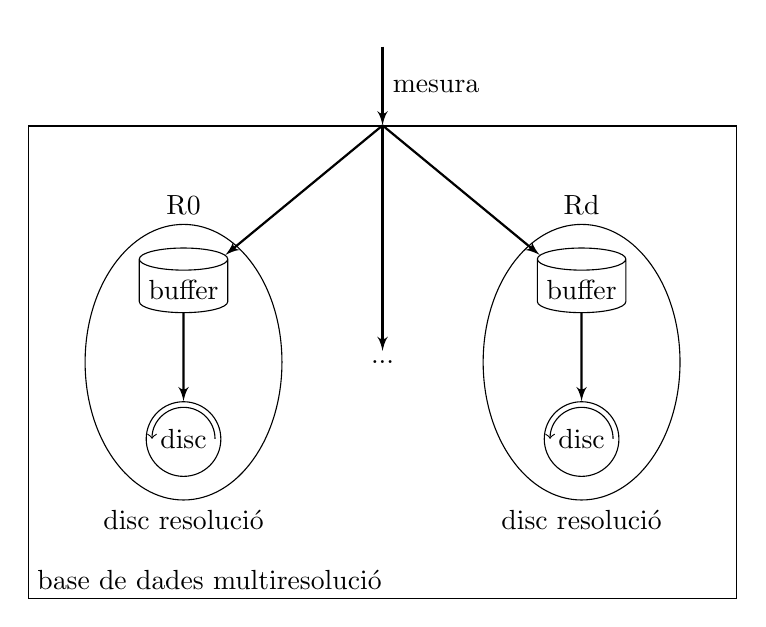
\begin{tikzpicture}
 \tikzset{
        myarrow/.style={->, >=latex',  thick},
      }
      

  \node[rectangle,draw,minimum height=6cm,minimum width=9cm] (m) {};
  \draw[shift=( m.south west)]   
  node[above right] {base de dades multiresolució};


  %discmig
  \node (m.center) (discr1) {...};

  %discr
  
  \node[ellipse,draw,minimum height=3.5cm,minimum width=2.5cm,alias=discr0] [left=of discr1] {};
  \node[above=0cm of discr0.north] {R0};
  \node[below=0cm of discr0] {disc resolució};

  \node[cylinder, draw, shape border rotate=90, aspect=0.25,alias=buffer0] [below=3mm of discr0.north] {buffer};
  \node[circle, draw,alias=disc0]  [above=3mm of discr0.south] {disc} ;
  \draw [->] (disc0.center)++(.4:.4cm) arc(0:180:.4cm);
  \draw[myarrow] (buffer0.bottom) -- (disc0.north);


  %discrd

  \node[ellipse,draw,minimum height=3.5cm,minimum width=2.5cm,alias=discrd] [right=of discr1] {};
  \node[above=0cm of discrd] {Rd};
  \node[below=0cm of discrd] {disc resolució};

  \node[cylinder, draw, shape border rotate=90, aspect=0.25,alias=bufferd] [below=3mm of discrd.north] {buffer};
  \node[circle, draw,alias=discd]  [above=3mm of discrd.south] {disc} ;
  \draw [->] (discd.center)++(.4:.4cm) arc(0:180:.4cm);
  \draw[myarrow] (bufferd.bottom) -- (discd.north);



  %mesura 
  \node[above=1cm of m.north] (m0) {};

  \draw[myarrow] (m0) -- (m.north) 
  node[right,midway] {mesura};

  \draw[myarrow] (m.north) -- (buffer0);
  \draw[myarrow] (m.north) -- (bufferd);
  \draw[myarrow] (m.north) -- (discr1);

\end{tikzpicture}
\caption{Arquitectura d'una BDSTM}
\label{fig:model:bdstm}
\end{figure}


Aquests objectes també permeten definir l'arquitectura d'una BDSTM com
es pot veure a la \autoref{fig:model:bdstm}.  Un SGSTM és una solució
d'emmagatzematge per a sèries temporals a on, resumint, la informació
es distribueix mitjançant diferents resolucions temporals.  Una sèrie
temporal multiresolució és una co\l.lecció de subsèries resolució, les
quals acumulen temporalment mesures en un buffer a on són processades
i finalment emmagatzemades en un disc. El processament de les dades té
per objectiu canviar els intervals de temps entre les mesures per tal
de compactar la informació de les sèries temporals. D'aquesta manera,
les sèries temporals queden emmagatzemades en diferents resolucions
temporals distribuïdes en els discs.

Els discs tenen la mida limitada i només poden contenir un nombre
fixat de mesures. Quan un disc no té més capacitat ha d'eliminar una
mesura. Com a conseqüència una BDSTM té la mida fixada i les sèries
temporals hi queden emmagatzemades a trossos; és a dir com a subsèries
temporals. 


En aquesta secció només es defineixen els conceptes referents a
l'estructura del model. Aquesta estructura, però, requereix uns
operadors específics per a emmagatzemar-hi i consolidar-hi les
mesures, els quals es defineixen a
l'apartat~\ref{sec:model:sgstm-estructurals}. També requereix unes
funcions per a agregar els atributs de les sèries temporals, els quals
es defineixen a l'apartat~\ref{sec:model:agregador}.




\subsection{Buffer}\label{sec:model:buffer}\todo{falta parlar de regularitat de ST}\todo{falta parlar de representació de ST}
\todo{que quedi clar que els buffers deleguen el càlcul a les $f$}

Un buffer és un contenidor d'una sèrie temporal, regular o no regular, que mitjançant una funció permet regularitzar aquesta sèrie temporal amb un període de mostreig constant. A l'acció de regularitzar un interval d'una sèrie temporal l'anomenarem consolidació, al període de mostreig contant l'anomenarem pas de consolidació i a la funció de regularització l'anomenarem agregador d'atributs.

\begin{definition}[Buffer]
  Definim \emph{buffer} com el tuple
  \glsdispdef{not:buffer}{$(S,\tau,\delta,f)$}, en el que
  \glsdispdef{not:sgstm:sb}{$S$} és una sèrie temporal,
  \glsdispdef{not:sgstm:tau}{$\tau$} és el darrer instant de temps de
  consolidació, \glsdispdef{not:sgstm:delta}{$\delta$} és la durada
  del pas de consolidació i \glsdispdef{not:sgstm:f}{$f$} és un
  agregador d'atributs.
\end{definition}

La consolidació d'una sèrie temporal s'inicia en un instant de temps
concret i té lloc a cada pas de consolidació. Amb la finalitat
d'establir els intervals de consolidació de la sèrie temporal, es
defineix un buffer inicial.

\begin{definition}\label{def:model:buffer_buit}
  Definim buffer inicial o buffer buit com el buffer $B_{\emptyset} =
  (\emptyset,t_0, \delta_0, f)$, el qual
  conté una sèrie temporal buida, l'instant de temps inicial de
  consolidació, una durada que indica el pas de consolidació i un
  agregador d'atributs.
\end{definition}

A partir del buffer buit es poden conèixer tots els instants de temps
de consolidació del buffer, els quals seran $t_0+k\delta,
k\in\mathbb{N}$. Aquests instants de temps de consolidació també
defineixen els intervals de temps de consolidació del buffer de la
forma $i=[\tau,\tau+\delta]$. La consolidació de la sèrie temporal $S$
d'un buffer en un interval de temps $i$ dóna com a resultat una mesura
$m=(t,v)$ calculada a partir de l'agregador d'atributs $m = f (S,
i)$. Més endavant a la \autoref{sec:model:agregador} detallem el
concepte d'agregador d'atributs.








\subsection{Disc}\label{sec:model:disc}

Un disc és un contenidor d'una sèrie temporal regular amb un nombre
acotat de mesures. En arribar al nombre màxim de mesures permeses,
cada cop que s'afegeix una mesura nova s'elimina la mesura mínima de
la sèrie temporal.  Així doncs, un disc és semblant a una cua
\emph{First In First Out} (FIFO), a on el primer d'arribar és el
primer de sortir.

\begin{definition}[Disc]
  Definim \emph{disc} com el tuple \glsdispdef{not:disc}{$(S,k)$}, en
  el que \glsdispdef{not:sgstm:sd}{$S$} és una sèrie temporal i
  \glsdispdef{not:sgstm:k}{$k\in\N{}$} és el cardinal màxim de $S$.
\end{definition}

A l'inici, un disc no conté mesures però cal que estigui caracteritzat
pel cardinal màxim. Amb aquesta finalitat es defineix un disc inicial.

\begin{definition}\label{def:model:disc_buit}
  Definim disc inicial o disc buit com el disc $D_{\emptyset} =
  (\emptyset,k)$, el qual conté una sèrie temporal buida i el cardinal
  màxim que podrà prendre $S$.
\end{definition}




\subsection{Subsèrie resolució}\label{sec:model:subserie-resolucio}

Una subsèrie temporal resolució és una parella de disc i buffer. En el
buffer hi ha la part d'una sèrie temporal a regularitzar i en el disc
hi ha l'altra part ja regularitzada, amb un nombre acotat de
mesures. A l'acció de regularitzar l'anomenem consolidar en coherència
amb el concepte descrit pels buffers.


\begin{definition}[Subsèrie resolució]
  Definim \emph{subsèrie resolució} com el tuple
  \glsdispdef{not:subserieresolucio}{$(B,D)$}, en el que $B$ és un buffer i $D$
  és un disc.
\end{definition}
 
La definició de buffer buit (def.~\ref{def:model:buffer_buit}) i de
disc buit (def.~\ref{def:model:disc_buit}) indueixen a una definició
de subsèrie resolució buida.
\begin{definition}\label{def:model:subserie_resolucio_buida}
  Definim subsèrie resolució buida com la subsèrie resolució $R_{\emptyset}
  = (B_{\emptyset},D_{\emptyset})$, la qual conté un buffer buit i un
  disc buit.
\end{definition}


Les subsèries resolució es consoliden seguint els criteris del seu
buffer i emmagatzemant la mesura de consolidació al seu disc.




\subsection{Sèrie temporal multiresolució}

Una sèrie temporal multiresolució és un conjunt de subsèries resolució que
comparteixen l'entrada de mesures, les quals provenen d'una mateixa
sèrie temporal. La sèrie temporal queda regularitzada i distribuïda en
les diferents subsèries resolució amb resolucions diferents, tal com s'ha
vist a la \autoref{fig:model:bdstm}


\begin{definition}[Sèrie temporal multiresolució]
  Definim \emph{sèrie temporal multiresolució} com el conjunt de subsèries
  resolució \glsdispdef{not:seriemultiresolucio}{$M=\{R_0,\dotsc,R_d\}$}.
\end{definition}

A partir de la definició de subsèrie resolució buida
(def.~\ref{def:model:subserie_resolucio_buida}) és defineix la sèrie
temporal multiresolució buida.
 
\begin{definition}\label{def:model:st_multiresolucio_buit}
  Definim sèrie temporal multiresolució buida com el conjunt de subsèries
  resolució buides
  $M_{\emptyset}=\{R_{0_{\emptyset}},\dotsc,R_{d_{\emptyset}\}}$.
\end{definition}

Normalment, en una sèrie temporal multiresolució no hi ha dues subsèries
resolució amb la mateixa informació. És a dir, donats dues subsèries
resolució $R_a = (B_a, D_a)$ i $R_b = (B_b, D_b)$, els seus respectius
buffers $B_a=(S_a,\tau_a,\delta_a,f_a)$ i
$B_b=(S_b,\tau_b,\delta_b,f_b)$ no tenen el mateix interval de
consolidació i agregador d'atributs: $\delta_a \neq \delta_b \wedge
f_a \neq f_b$.




\subsection{Base de dades de sèries temporals
  multiresolució}\label{sec:model:bdstm}

Una base de dades de sèries temporals multiresolució (BDSTM) és una
co\l.lecció de sèries temporal multiresolució.  Les sèries temporals
es poden emmagatzemar exclusivament en una BDSTM o poden conviure amb
altres tipus de dades en bases de dades que tinguin capacitats de
BDSTM.


Una BDSTM té uns paràmetres que cal configurar per a cada sèrie
temporal multiresolució: pas de consolidació, funció d'agregació,
etc. Anomenem esquema de multiresolució a l'efecte que produeixen les
configuracions possibles d'aquests paràmetres. Així doncs, a cada
BDSTM li podem observar i manipular els seus esquemes de
multiresolució, el qual mostrem amb més detall a
l'apartat~\ref{sec:model:sgstm-manipulacio-esquema}.



\subsubsection{Relació sèrie temporal multiresolució}


Una sèrie temporal multiresolució és una relació de buffers i discs. A
cada parella buffer-disc l'anomenem subsèrie resolució. Així doncs, una
sèrie temporal multiresolució és un conjunt de subsèries resolució.

Com a conjunt de subsèries resolució, una sèrie temporal multiresolució
s'observa com una relació de grau sis a on la capçalera conté els
atributs
\begin{itemize}
\item sèrie temporal del buffer ($S_B$),
\item sèrie temporal del disc ($S_D$),
\item darrer instant de consolidació ($\tau$),
\item pas de consolidació ($\delta$),
\item màxim cardinal del disc ($k$),
\item i funció d'agregació d'atributs ($f$).
\end{itemize}

Una restricció habitual és que $\delta$ i $f$ no estiguin repetits; és
a dir que ($\delta$,$f$) són els atributs clau de la relació sèrie
temporal multiresolució.

Així doncs observada com a relació, tal com s'ha fet en el model de
SGST, podem escriure una sèrie temporal multiresolució
\begin{definition}[Representació sèrie temporal multiresolució]
  Sigui $M=\{R_0,\dotsc,R_d\}$ una sèrie temporal multiresolució a on
  $R_i =(B_i,D_i)$ són subsèries resolució amb domini de sèrie
  temporal per les sèries temporals, de $\bar{\R{}}$ pels temps, de
  $\N{}$ pel pas de consolidació i de funció per a la funció
  d'agregació d'atributs;
  \glsdispdef{not:sgstm:relaciomultiresolucio}{representada com a relació}
  s'escriu com $ M = ( S_B: \text{Sèrie Temporal}, S_D: \text{Sèrie
    Temporal}, \tau: \R{}, \delta: \R{}, k: \N{}, f: \text{funció}\},
  \{ \{ S_B: S_{B_0} , S_D : S_{D_0} , \tau : \tau_{B_0}, \delta :
  \delta_{B_0}, k: k_{D_0}, f : f_{B_0} \} , \dotsc, \{ S_B: S_{B_d} ,
  S_D : S_{D_d} , \tau : \tau_{B_d}, \delta : \delta_{B_d}, k:
  k_{D_d}, f : f_{B_d} \} \} )$.
\end{definition}

De la mateixa manera que per a les sèries temporals en el model de
SGST, una sèrie temporal multiresolució es pot escriure de manera
simplificada com al conjunt de tuples $M = \{ (S_{B_0}, S_{D_0} ,
\tau_{B_0}, \delta_{B_0}, k_{D_0}, f_{B_0} ), \dotsc, (S_{B_d},
S_{D_d} , \tau_{B_d}, \delta_{B_d}, k_{D_d}, f_{B_d} ) \}$.




\subsection{Exemples}

\begin{example} [Sèrie temporal multiresolució]
\label{ex:model:bdm1}%ATENCIÓ als canvis: les dades d'aquest exemple s'utilitzen en altres apartat.


Sèrie temporal multiresolució $M_1=\{R_0,R_1\}$ que té dues subsèries
resolució amb els paràmetres següents:
\begin{itemize}
\item La subsèrie resolució $R_0$ té un pas de consolidació de 5
  unitats de temps, una mida màxima de 4 mesures i una funció de
  consolidació de 'mitjana' de les mesures.
\item La subsèrie resolució $R_1$ té un pas de consolidació de 10
  unitats de temps, una mida màxima de 3 mesures i una funció de
  consolidació de 'mitjana' de les mesures.
\end{itemize}

\begin{figure}[tp]
\centering
%\usetikzlibrary{shapes,arrows,positioning}
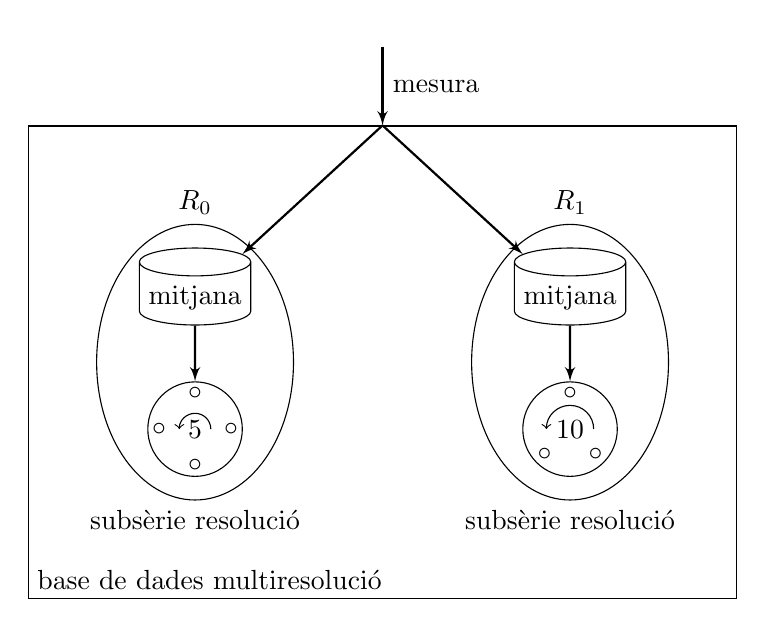
\begin{tikzpicture}
 \tikzset{
        myarrow/.style={->, >=latex',  thick},
      }
      

  \node[rectangle,draw,minimum height=6cm,minimum width=9cm] (m) {};
  \draw[shift=( m.south west)]   
  node[above right] {base de dades multiresolució};


  %discmig
  \node (m.center) (discr1) {};

  %discr
  
  \node[ellipse,draw,minimum height=3.5cm,minimum width=2.5cm,alias=discr0] [left=of discr1] {};
  \node[above=0cm of discr0.north] {$R_0$};
  \node[below=0cm of discr0] {subsèrie resolució};

  \node[cylinder, draw, shape border rotate=90, aspect=0.25,alias=buffer0] [below=3mm of discr0.north] {mitjana};
  \node[circle, draw,alias=disc0,minimum width=1.2cm]  [above=3mm of discr0.south] {5} ;
  \draw [->] (disc0.center)++(.2:.2cm) arc(0:180:.2cm);
  \draw[myarrow] (buffer0.bottom) -- (disc0.north);

  \node[circle,minimum width=9mm] (d0boles) [below=0mm of disc0.center,anchor=center] {};
  \node[below=0mm of d0boles.north,anchor=center] {$\circ$};
  \node[below=0mm of d0boles.east,anchor=center] {$\circ$};
  \node[below=0mm of d0boles.south,anchor=center] {$\circ$};
  \node[below=0mm of d0boles.west,anchor=center] {$\circ$};


  %discrd

  \node[ellipse,draw,minimum height=3.5cm,minimum width=2.5cm,alias=discrd] [right=of discr1] {};
  \node[above=0cm of discrd] {$R_1$};
  \node[below=0cm of discrd] {subsèrie resolució};

  \node[cylinder, draw, shape border rotate=90, aspect=0.25,alias=bufferd] [below=3mm of discrd.north] {mitjana};
  \node[circle, draw,alias=discd,minimum width=1.2cm]  [above=3mm of discrd.south] {10} ;
  \draw [->] (discd.center)++(.3:.3cm) arc(0:180:.3cm);
  \draw[myarrow] (bufferd.bottom) -- (discd.north);

  \node[circle,minimum width=9mm] (d1boles) [below=0mm of discd.center,anchor=center] {};
  \node[below=0mm of d1boles.north,anchor=center] {$\circ$};
  \node[below=0mm of d1boles.south east,anchor=center] {$\circ$};
  \node[below=0mm of d1boles.south west,anchor=center] {$\circ$};


  %mesura 
  \node[above=1cm of m.north] (m0) {};

  \draw[myarrow] (m0) -- (m.north) 
  node[right,midway] {mesura};

  \draw[myarrow] (m.north) -- (buffer0);
  \draw[myarrow] (m.north) -- (bufferd);


\end{tikzpicture}
\caption{Arquitectura de SGSTM particular per l'\autoref{ex:model:bdm1}}
\label{fig:model:ex1}
\end{figure}

L'arquitectura de la base de dades que conté aquesta sèrie temporal
multiresolució es pot veure a la \autoref{fig:model:ex1}. 
 L'esquema
de multiresolució que correspon als instants de consolidació, des de 0
fins a 30, és el següent:
\begin{itemize}
\item La subsèrie resolució $R_0$ serà consolidada en els instants 5,
  10, 15, 20, 25 i 30.
\item La subsèrie resolució $R_1$ serà consolidada en els instants 10,
  20 i 30.
\end{itemize}


Iniciem la base de dades a l'instant de temps 0, instant en el qual la
sèrie temporal multiresolució és $M_1^0 = \{ ( \{\} , \{\} , 0 , 5 ,4
, \text{mitjana} ) , ( \{\} , \{\} , 0 , 10 ,3 , \text{mitjana} ) \}$;
és a dir amb les sèries temporals buides i els darrers instants de
consolidació iniciats a 0.




A continuació, afegim a la sèrie temporal multiresolució les mesures
de la sèrie temporal $S_1=\{
(1,0),(5,0),(8,0),(10,0),(14,0),(19,0),(22,0),(26,0),(29,0) \}$. Tots
els valors valen zero per tal de centrar la comprensió de l'exemple en
l'estructura de temps de consolidació; pel que fa a exemples
d'agregació de valors es poden veure amb més detall a la
secció~\ref{sec:model:agregador}.


Si consolidem la sèrie temporal multiresolució cada cop que sigui
consolidable, és a dir en els instants que marca l'esquema de
multiresolució, a l'instant 29 després d'haver inserit la darrera
mesura la sèrie temporal multiresolució és $M_1^{29} = \{ (
\{(26,0),(29,0)\},\{(10,0),(15,0),(20,0),(25,0)\}, 25 , 5 ,4 ,
\text{mitjana} ), ( \{(22,0),(26,0),(29,0)\}, \{(10,0),(20,0)\},
20 , 10 ,3 , \text{mitjana} ) \}$.  Aquesta sèrie temporal
multiresolució es mostra a la \autoref{fig:model:stm} en forma de
taula.


Es pot observar que als buffers hi ha emmagatzemades les mesures
pendents de consolidar per a cada subsèrie i als discs les darreres
mesures consolidades:
\begin{itemize}
\item Per a la subsèrie resolució $R_0$ hi ha pendent de consolidar
  l'interval de temps $[25,30]$ i al disc hi ha emmagatzemades les 4
  mesures màximes permeses; és a dir que la que s'havia consolidat a
  l'instant $5$ ja s'ha perdut.
\item Per a la subsèrie resolució $R_1$ hi ha pendent de consolidar
  l'interval de temps $[20,30]$ i al disc hi ha emmagatzemades 2
  mesures. El disc encara no ha arribat al cardinal màxim $k=3$ degut
  a que la base de dades s'ha iniciat a l'instant $0$ i la primera
  consolidació d'aquesta subsèrie ha estat a l'instant $10$.
\end{itemize}




\begin{figure}[tp]
  \centering
  \begin{tabular}{|c|c|c|c|c|c|}
    \multicolumn{2}{c}{$M_1^{29}$} \\ \hline
    $S_B$  & $S_D$ & $\tau$ & $\delta$ & $k$ & $f$ \\ \hline
      \begin{tabular}{|c|c|}
         \hline
         $t$  & $v$ \\ \hline
         26  & 0 \\
         29 & 0 \\\hline
       \end{tabular} & 
      \begin{tabular}{|c|c|}
         \hline
         $t$  & $v$ \\ \hline
         10  & 0 \\
         15  & 0 \\
         20 & 0 \\ 
         25 & 0 \\\hline
       \end{tabular} 
       & 25 & 5  & 4 & mitjana  \\ \hline
       \begin{tabular}{|c|c|}
         \hline
         $t$  & $v$ \\ \hline
         22  & 0 \\
         26  & 0 \\
         29 & 0 \\\hline
       \end{tabular} & 
      \begin{tabular}{|c|c|}
         \hline
         $t$  & $v$ \\ \hline
         10  & 0 \\
         20  & 0 \\\hline
       \end{tabular}  
       & 20 & 10 & 3 & mitjana  \\ \hline
  \end{tabular}
  \caption{Taula d'una sèrie temporal multiresolució}
  \label{fig:model:stm}
\end{figure}

\end{example}


\begin{example} [Sèrie temporal multiresolució amb vistes]

  En el model relacional de SGBD molt sovint s'utilitzen vistes per a
  agrupar informació de vàries relacions, per a mostrar-ne una part,
  etc. Una vista és una variable relació virtual derivada d'una
  expressió relacional \parencite{date13}. En aquest exemple mostrem
  la mateixa sèrie temporal multiresolució de
  l'\autoref{ex:model:bdm1} però organitzada amb forma de vistes
  relacionals.


  Sigui $M_2^{\text{series}}= ((S':\text{nom},S:\text{sèrie
    temporal}),\{ (S_{B1},\{(26,0),(29,0)\}),
  (S_{B2},\{(22,0),(26,0),(29,0)\}),
  (S_{D1},\{(10,0),(15,0),(20,0),(25,0)\}),
  (S_{D2},\{(10,0),(20,0)\} )\})$ una relació de sèries
  temporals i noms, i $M_2'=
  ((S'_B:\text{nom},S'_D:\text{nom},\tau:\R,\delta:\R,k:\N,f:\text{funció}
  ),\{ (S_{B1},S_{D1},25 ,5 ,4 ,\text{mitjana} ), ( S_{B2},S_{D2},20 ,
  10 ,3 , \text{mitjana} ) \})$ una sèrie temporal multiresolució amb
  noms als atributs de sèries temporals; la vista de la sèrie temporal
  multiresolució es mostra a la \autoref{fig:model:stm:vistes} i es
  defineix com a
  \begin{align*}
    \text{vista } M_2 =& (M_2' \join ( M_2^{\text{series}} \rename S' \as S_B', S \as S_B )) \\
    &\join ( M_2^{\text{series}} \rename S' \as S_D', S \as S_D )
    \{\text{all but } S_B',S_D' \}
  \end{align*}




  \begin{figure}[tp]
    \centering
    \begin{tabular}{|c|c|c|c|c|c|}
      \multicolumn{2}{c}{$M'_2$} \\ \hline
      $S'_B$  & $S'_D$ & $\tau$ & $\delta$ & $k$ & $f$ \\ \hline
      $S_{B1}$ & $S_{D1}$ & 25 & 5  & 4 & mitjana  \\
      $S_{B2}$ & $S_{D2}$ & 20 & 10 & 3 & mitjana  \\ \hline
    \end{tabular}\qquad
    \begin{tabular}{|c|c|c|}
      \multicolumn{3}{c}{$M^{\text{series}}_{2}$} \\ \hline
      \multirow{2}{*}{$S'$}  &  \multicolumn{2}{c|}{$S$} \\ \cline{2-3}
      & $t$      & $v$  \\ \hline
      \multirow{2}{*}{$S_{B1}$} 
      & 26 & 0 \\ 
      & 29 & 0 \\ \hline
      \multirow{3}{*}{$S_{B2}$} 
      & 22 & 0 \\ 
      & 26 & 0 \\ 
      & 29 & 0 \\ \hline
      \multirow{4}{*}{$S_{D1}$} 
      & 10 & 0 \\ 
      & 15 & 0 \\ 
      & 20 & 0 \\ 
      & 25 & 0 \\ \hline
      \multirow{2}{*}{$S_{D2}$} 
      & 10 & 0 \\ 
      & 20 & 0 \\ \hline
    \end{tabular}
    \caption{Taula d'una sèrie temporal multiresolució amb vistes
      relacionals}
    \label{fig:model:stm:vistes}
  \end{figure}


  D'aquesta manera $M_2$ té els mateixos valors que la $M_1$ definida
  a l'exemple anterior; observant només el resultat de $M_2$ no es pot
  distingir que és una vista. Així doncs, les vistes ens permeten
  organitzar una sèrie temporal multiresolució de forma més còmoda i,
  a més tal com es descriu a \textcite{date13}, mantenint que totes
  les operacions i propietats que són d'aplicació a les relacions ho
  són també a les seves vistes.


%S'observa que per tal de complir amb les propietats de les relacions, totes les sèries temporals dels buffers han de ser del mateix tipus, és a dir tenir la mateixa capçalera. El mateix succeeix amb les sèries temporals dels discs. (Vegeu els exemples de la secció \ref{par:model:exemple-relvalues} sobre valors relació). No obstant les mesures que entren a la base de dades provenen de la mateixa sèrie temporal i per tant les sèries temporals emmagatzemades sempre seran del mateix tipus.



\end{example}



\begin{example} [Sèrie temporal multiresolució amb desfasaments]
\label{ex:model:bdm-desfasaments}

A l'\autoref{ex:model:bdm1} s'ha mostrat una sèrie temporal
multiresolució en la que la consolidació de les dues subsèries obeeix
a la mateixa funció d'agregador d'atributs $f$. En aquest exemple
treballem amb els mateixos valors que a l'\autoref{ex:model:bdm1} però
ara canviem la funció de la segona subsèrie resolució per un agregador
amb desfasament; és a dir que cada cop que consolida retorna una
mesura amb un retard d'una certa durada. Aquest nou agregador que
anomenem \emph{mitjanad5} també fa la mitjana però amb un desfasament
de $5$ unitat de temps, a l'apartat
\ref{sec:model:sgstm-manipulacio-esquema} es defineix amb més precisió
aquest concepte de desfasament.


Seguint el mateix procediment que a l'\autoref{ex:model:bdm1}, a
l'instant 29 després d'haver inserit la darrera mesura la sèrie
temporal multiresolució és $M_3^{29} = \{ ( \{(26,0),(29,0)\} ,
\{(10,0),(15,0),(20,0),(25,0)\} , 25 , 5 ,4 , \text{mitjana} ) , (
\{(19,0),(22,0),(26,0),(29,0)\} , \{(5,0),(15,0)\} , 20 , 10 ,3 ,
\text{mitjanad5} ) \}$.  Aquesta sèrie temporal multiresolució es
mostra a la \autoref{fig:model:stm:desfasaments} en forma de taula.


\begin{figure}[tp]
  \centering
  \begin{tabular}{|c|c|c|c|c|c|}
    \multicolumn{2}{c}{$M_3^{29}$} \\ \hline
    $S_B$  & $S_D$ & $\tau$ & $\delta$ & $k$ & $f$ \\ \hline
      \begin{tabular}{|c|c|}
         \hline
         $t$  & $v$ \\ \hline
         26  & 0 \\
         29 & 0 \\\hline
       \end{tabular} & 
      \begin{tabular}{|c|c|}
         \hline
         $t$  & $v$ \\ \hline
         10  & 0 \\
         15  & 0 \\
         20 & 0 \\ 
         25 & 0 \\\hline
       \end{tabular} 
       & 25 & 5  & 4 & mitjana  \\ \hline
       \begin{tabular}{|c|c|}
         \hline
         $t$  & $v$ \\ \hline
         19  & 0 \\
         22  & 0 \\
         26  & 0 \\
         29 & 0 \\\hline
       \end{tabular} & 
      \begin{tabular}{|c|c|}
         \hline
         $t$  & $v$ \\ \hline
          5  & 0 \\
         15  & 0 \\\hline
       \end{tabular}  
       & 20 & 10 & 3 & mitjanad5  \\ \hline
  \end{tabular}
  \caption{Taula d'una sèrie temporal multiresolució amb desfasaments}
  \label{fig:model:stm:desfasaments}
\end{figure}



Així doncs, mentre que l'esquema de multiresolució segueix sent el
mateix pel que fa als instants de consolidació, els instants de temps
de la sèrie temporal emmagatzemada a la subsèrie resolució $R_1$ tenen
un retard de $5$ unitats de temps.  Per una banda, es pot observar a
la $S_{B2}$ que el buffer ara és 5 unitats més gran i emmagatzema
mesures de l'interval $[15,30]$. Per altra banda, es pot observar a la
$S_{D2}$ que els instants emmagatzemats són $5$ i $15$ corresponents
als instants de consolidació $10$ i $20$. Pel que fa a la resta de
valors, no han variat respecte de l'\autoref{ex:model:bdm1}.



\end{example}


%%% Local Variables: 
%%% mode: latex
%%% TeX-master: "main"
%%% End: 

% LocalWords:  buffers multiresolució agregador l'agregador subsèries
% LocalWords:  d'agregador








\begin{frame}<handout:0>
  \addtocounter{framenumber}{-1}

  \begin{center}
    {\huge
      Gràcies per l'atenció!
    }
  \end{center}

\end{frame}


\appendix


\begin{frame}[allowframebreaks]{Referències}

\printbibliography

\end{frame}


\end{document}


%%%%%%%%%%%%%%%%%%%%%%%%%%%%%%%%%%%%%%%%%%%%%%%%%%%%%%%%%%%%%%%%%%%%%%%%%%  
% Defensa Tesi Doctoral. 
%
% Copyright (C) 2011-2015 Aleix Llusà Serra.
% 
% This LaTeX document is free software: you can redistribute it and/or
% modify it under the terms of the GNU General Public License as
% published by the Free Software Foundation, either version 3 of the
% License, or (at your option) any later version.
%
% This document is distributed in the hope that it will be useful, but
% WITHOUT ANY WARRANTY; without even the implied warranty of
% MERCHANTABILITY or FITNESS FOR A PARTICULAR PURPOSE. See the GNU
% General Public License for more details.
%
% You should have received a copy of the GNU General Public License
% along with this document. If not, see <http://www.gnu.org/licenses/>.
%
%
% Aleix Llusà Serra
% Departament de Disseny i Programació de Sistemes Electrònics de la Universitat Politècnica de Catalunya (DiPSE-UPC)
% Escola Politècnica Superior d'Enginyeria de Manresa (EPSEM)
% Av. de les Bases de Manresa, 61-73
% 08242 Manresa (Barcelona)
% PAÏSOS CATALANS 
%
% aleix (a) dipse.upc.edu
% 
% El codi font LaTeX del document es troba a 
% <http://escriny.epsem.upc.edu/projects/rrb/>
%%%%%%%%%%%%%%%%%%%%%%%%%%%%%%%%%%%%%%%%%%%%%%%%%%%%%%%%%%%%%%%%%%%%%%%%%% 